% % \part{数学建模实战}
% % \chapter{嫦娥3号}

% \documentclass[UTF8]{ctexbook}

% \ctexset{
%     part/number = \chinese{part}
% }

% \usepackage{multirow}
% \usepackage{amsmath}% ams 数学公式
% \usepackage{amsfonts}% ams 数学字体
% \usepackage{bbm}%重影字体
% \usepackage{amssymb,latexsym}% ams 数学符号与LaTeX数学符号
% \usepackage{mathrsfs}% 花式符号
% \usepackage{ntheorem}%定理、定义、证明
%     \theoremstyle{nonumberplain}
%     \theoremheaderfont{\bfseries}
%     \theorembodyfont{\normalfont}
%     \theoremsymbol{$\square$}
%     \newtheorem{Proof}{\hskip 2em 证明}
%     \newtheorem{theorem}{\hspace{2em}定理}[chapter]
%     \newtheorem{definition}{\hspace{2em}定义}[chapter] % 如果没有章, 只有节, 把上面的[chapter]改成[section]
%     \newtheorem{axiom}[definition]{\hspace{2em}公理}
%     \newtheorem{lemma}[definition]{\hspace{2em}引理}
%     \newtheorem{proposition}[definition]{\hspace{2em}命题}
%     \newtheorem{corollary}[definition]{\hspace{2em}推论}
%     \newtheorem{remark}{\hspace{2em}注}[chapter] %类似地定义其他“题头”. 这里“注”的编号与定义、定理等是分开的
%     \newtheorem{Assumption}{\hspace{2em}假设}[chapter]

% %算法伪代码
% %http://blog.csdn.net/lwb102063/article/details/53046265
% \usepackage{algorithm}
% \usepackage{algorithmicx}
% \usepackage{algpseudocode}
%     \floatname{algorithm}{算法}
%     \renewcommand{\algorithmicrequire}{\textbf{输入:}}
%     \renewcommand{\algorithmicensure}{\textbf{输出:}}
% % 罗马数字:示例:\rom{2}
% \makeatletter
% \newcommand*{\rom}[1]{\expandafter\@slowromancap\romannumeral #1@}
% \makeatother

% \usepackage{enumerate}%itemiz环境。\begin{enumerate}[step 1][a)]可以使用 A,a,I,i,1 作为可选项产生 \Alph,\alph,\Roman,\roman,\arabic 的效果
% \usepackage{cite}%参考文献
%     \bibliographystyle{plain}
% \usepackage{extarrows}% 带参数的箭头
% \usepackage{hyperref}% 超链接
% \usepackage{pifont}%然后在正文输入\ding{172}~\ding{211}得到相应数字,要是要①就输入:\ding{172}②就输:\ding{173}
% %\usepackage[CJKbookmarks, colorlinks, bookmarksnumbered=true,pdfstartview=FitH,linkcolor=black,citecolor=black]{hyperref}%超链接的格式设置
% \hypersetup{
%     colorlinks=false,% 去掉超链接颜色
%     pdfborder=0 0 0% 取消超链接的边框
% }
% \usepackage{graphicx}% 图片管理
% \usepackage{caption}
% \usepackage{subcaption}%并排的图各有标题
% \graphicspath{{images/}}% 设置图片搜索路径
% \usepackage{float,varwidth}% 浮动体
% \usepackage{booktabs}% 三线表
% \usepackage{fancyhdr}% 页眉设置
% \usepackage{xcolor}% 颜色宏包
% \usepackage{colortbl}% 彩色表格
% \usepackage{listings}% 代码高亮
% \usepackage{caption}% 对标题进行控制,如让\caption标题的字体缩小一号,同时数字标签使用粗体可以用:\usepackage[font=small,labelfont=bf]{caption}
% \usepackage{xfrac,upgreek}%分别是行间公式如a/b的形式(将原来的命令\frac改成\sfrac)和希腊字体的宏包的
% \usepackage{mathtools}%lgathered和rgathered环境把公式向左向右对齐
% \usepackage{tabularx}%提供自动延伸的表列,(X列格式说明符),文字过长时可以自动转行
% \usepackage{longtable}%长表格
% \usepackage{enumitem}%enumerate宏包的升级
% \usepackage{harpoon}%数学公式的矢量
% \usepackage{bookmark}%目录的书签
% \renewcommand{\headwidth}{\textwidth}%图片并排,这个要列在所有宏包的后面
% \definecolor{codegreen}{rgb}{0,0.6,0}
% \definecolor{codegray}{rgb}{0.5,0.5,0.5}
% \definecolor{codepurple}{rgb}{0.58,0,0.82}
% \definecolor{backcolour}{rgb}{0.95,0.95,0.92}
% \lstset{
%     commentstyle=\color{codegreen},
%     keywordstyle=\color{magenta},
%     numberstyle=\tiny\color{codegray},
%     stringstyle=\color{codepurple},
%     basicstyle=\footnotesize,
%     breakatwhitespace=false,% 断行只在空格处
%     breaklines=true,% 自动断行
%     captionpos=b,% 标题位置
%     keepspaces=true,
%     numbers=left,
%     numbersep=5pt,
%     showspaces=false,
%     showstringspaces=false,
%     showtabs=false,% 显示
%     tabsize=2% TAB 被当作两个空格
% }
% \topmargin=0pt\oddsidemargin=0pt\evensidemargin=0pt
% \textwidth=16.5cm\textheight=23cm\raggedbottom%我这么设置是为了缩小页边距,满足有的文字无法转行
% \pagestyle{headings}%页眉为章节标题,无页脚
% \setlength{\abovecaptionskip}{10pt}
% \setlength{\belowcaptionskip}{-15pt}%图片表格的前后距离设置
% \CTEXsetup[format={\zihao{-3}\raggedright\bfseries}]{section}%设置节的格式

% \begin{document}
% \part{数学建模实战}
\chapter{嫦娥3号}
\section{题目要求}
    \par
    \textbf{A题:嫦娥三号软着陆轨道设计与控制策略}\footnote{2014高教社杯全国大学生数学建模竞赛题目}
    \par
    嫦娥三号于2013年12月2日1时30分成功发射,12月6日抵达月球轨道。嫦娥三号在着陆准备轨道上的运行质量为$2.4t$,其安装在下部的主减速发动机能够产生$1500N$到$7500N$的可调节推力,其比冲(即单位质量的推进剂产生的推力)为$2940m/s$,可以满足调整速度的控制要求。在四周安装有姿态调整发动机,在给定主减速发动机的推力方向后,能够自动通过多个发动机的脉冲组合实现各种姿态的调整控制。嫦娥三号的预定着陆点为$19.51W$,$44.12N$,海拔为$-2641m$(见附件1)。
    \par
    嫦娥三号在高速飞行的情况下,要保证准确地在月球预定区域内实现软着陆,关键问题是着陆轨道与控制策略的设计。其着陆轨道设计的基本要求:着陆准备轨道为近月点$15km$,远月点$100km$的椭圆形轨道;着陆轨道为从近月点至着陆点,其软着陆过程共分为6个阶段(见附件2),要求满足每个阶段在关键点所处的状态;尽量减少软着陆过程的燃料消耗。
    \par
    根据上述的基本要求,请你们建立数学模型解决下面的问题:
    \par
    (1)确定着陆准备轨道近月点和远月点的位置,以及嫦娥三号相应速度的大小与方向。
    \par
    (2)确定嫦娥三号的着陆轨道和在6个阶段的最优控制策略。
    \par
    (3)对于你们设计的着陆轨道和控制策略做相应的误差分析和敏感性分析。
    \subsection{附件1:问题的背景与参考资料;}
        \subsubsection{1.中新网12月12日电(记者 姚培硕)}
            \par
            根据计划\footnote{http://www.chinanews.com/mil/2013/12-12/5608941.shtml},嫦娥三号将在北京时间12月14号在月球表面实施软着陆。嫦娥三号如何实现软着陆以及能否成功成为外界关注的焦点。目前,全球仅有美国、前苏联成功实施了13次无人月球表面软着陆。
            \par
            北京时间12月10日晚,嫦娥三号已经成功降轨进入预定的月面着陆准备轨道,这是嫦娥三号“落月”前最后一次轨道调整。在实施软着陆之前,嫦娥三号还将在这条近月点高度约15公里、远月点高度约100公里的椭圆轨道上继续飞行。期间,将稳定飞行姿态,对着陆敏感器、着陆数据等再次确认,并对软着陆的起始高度、速度、时间点做最后准备。
            \par
            “发射、近月制动、变轨和月面降落比较起来,后者更为关键。这对我们来说是一个全新的,也是一个最重要的考验。”中国探月工程总设计师吴伟仁表示。
            \par
            嫦娥三号着陆地点选在较为平坦的虹湾区。但由于月球地形的不确定性,最终“落月”地点的选择仍存在一定难度。据悉,嫦娥三号将在近月点15公里处以抛物线下降,相对速度从每秒1.7公里逐渐降为零。整个过程大概需要十几分钟的时间。探测器系统副总指挥谭梅将其称为“黑色750秒”。
            \par
            由于月球上没有大气,嫦娥三号无法依靠降落伞着陆,只能靠变推力发动机,才能完成中途修正、近月制动、动力下降、悬停段等软着陆任务。据了解,嫦娥三号主发动机是目前中国航天器上最大推力的发动机,能够产生从1500牛到7500牛的可调节推力,进而对嫦娥三号实现精准控制。
            \par
            在整个“落月”过程中,“动力下降”被业内形容为最惊心动魄的环节。在这个阶段,嫦娥三号要完全依靠自主导航控制,完成降低高度、确定着陆点、实施软着陆等一系列关键动作,人工干预的可能性几乎为零。“在这个时间段内测控都跟不上了,判断然后上去执行根本来不及,只能事先把程序都设定好。”谭梅表示。
            \par
            在距月面100米处时,嫦娥三号要进行短暂的悬停,扫描月面地形,避开障碍物,寻找着陆点。“如果下面有个大坑,需要挪个地方,它就会自己平移,等照相机告诉它地面平了,才会降落”。中国绕月探测工程首任首席科学家、中国科学院院士欧阳自远介绍。
            \par
            之后,嫦娥三号在反推火箭的作用下继续慢慢下降,直到离月面4米高时再度悬停。此时,关掉反冲发动机,探测器自由下落。由于探测器具备着陆缓冲机构,几个腿都有弹性,落地时不至于摔坏。
            \par
            安全降落以后,嫦娥三号将打开太阳能电池板接收能量,携带的仪器经过测试、调试后开始工作。随后,“玉兔号”月球车将驶离着陆器,在月面进行3个月的科学勘测,着陆器则在着陆地点进行原地探测。这将是中国航天器首次在地外天体的软着陆和巡视勘探,同时也是1976年后人类探测器首次的落月探测。
        \subsubsection{2.嫦娥三号近月轨道示意图(曲振东 编制)}
            \par
            \begin{figure}[H]
            \centering
            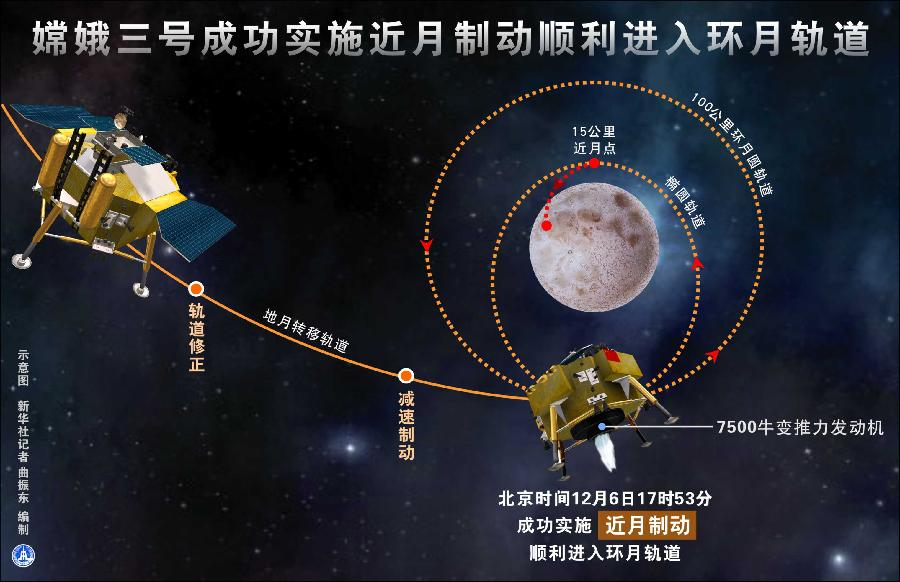
\includegraphics[width = 8cm]{images/near_track.png}
            \caption{嫦娥三号近月轨道示意图}\footnote{http://news.xinhuanet.com/photo/2013-12/02/c$\_$125789895.htm}
            \label{fig:嫦娥三号近月轨道示意图}
            \end{figure}
        \subsubsection{3.嫦娥三号着陆区域和着陆点示意图}
            \par
            \begin{figure}[H]
            \centering
            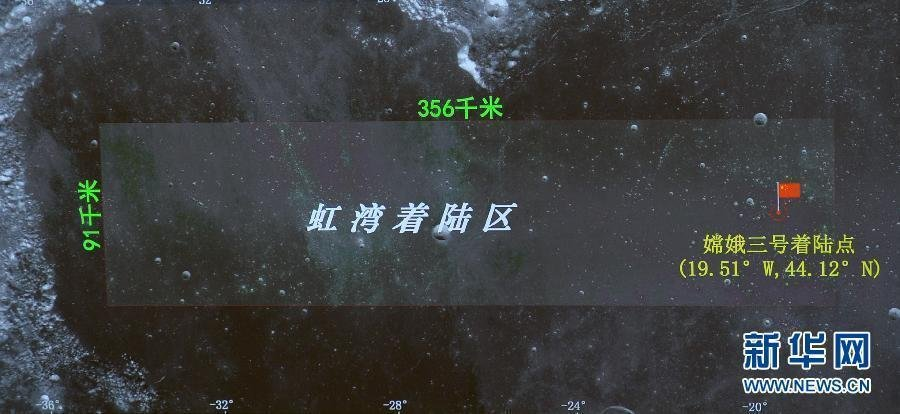
\includegraphics[height=4cm]{images/Landing_area_and_landing_point.jpg}
            \caption{嫦娥三号着陆区域和着陆点示意图}\footnote{http://blog.guandian.cn/?p=83491}
            \label{fig:嫦娥三号着陆区域和着陆点示意图}
            \end{figure}
        \subsubsection{4.主发动机和姿态调整发动机的分布图}
            \par
            嫦娥三号安装有大推力主减速发动机一台,位于正下方。小型姿态调整发动机16台,分布在相对前、后、左、右四个侧面,如图(\ref{fig:嫦娥三号主发减速动机与姿态调整发动机的分布图})是一个侧面的分布情况。
            \begin{figure}[H]
            \centering
            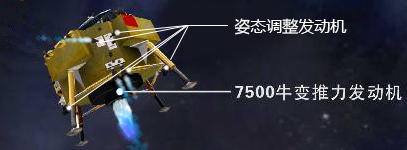
\includegraphics[height=4cm]{images/Main_engine_deceleration_motive.jpg}
            \caption{嫦娥三号主发减速动机与姿态调整发动机的分布图}
            \label{fig:嫦娥三号主发减速动机与姿态调整发动机的分布图}
            \end{figure}
        \subsubsection{5.关于比冲}
            \par
            比冲\footnote{维基百科,比冲. http://en.wikipedia.org/wiki/Specific$\_$impulse. 2014.1.17}或比冲量是对一个推进系统的燃烧效率的描述。比冲的定义为:火箭发动机单位质量推进剂产生的冲量,或单位流量的推进剂产生的推力。比冲的单位为米/秒(m/s),并满足下列关系式:
            \begin{align*}
            F_{thrust} = v_e\dot{m}
            \end{align*}
            其中:$F_{thrust}$是发动机的推力,单位是牛顿;$v_e$是以米/秒为单位的比冲;$\dot{m}$是单位时间燃料消耗的公斤数。
        \subsubsection{6.关于月球参数}
            \par
            月球平均半径、赤道平均半径和极区半径分别为$1737.013km$、$1737.646km$和$1735.843km$,月球的形状扁率为$1/963.7256$,月球质量是$7.3477\times 1022kg$。月球与地球距离最远(远地点):$406610km$,最近(近地点):$356330km$,平均距离为$384400km$。
            \par
            NASA月球勘测轨道飞行器使用的月面海拔零点,是月球的平均半径所在的高度。所以,嫦娥三号着陆点的海拔为$-2640m$,即该点到月球中心的距离要比月球的平均半径少$2640m$。
    \subsection{附件2:嫦娥三号着陆过程的六个阶段及其状态要求;}
        \subsubsection{1. 嫦娥三号软着陆过程示意图}
            \begin{figure}[H]
            \centering
            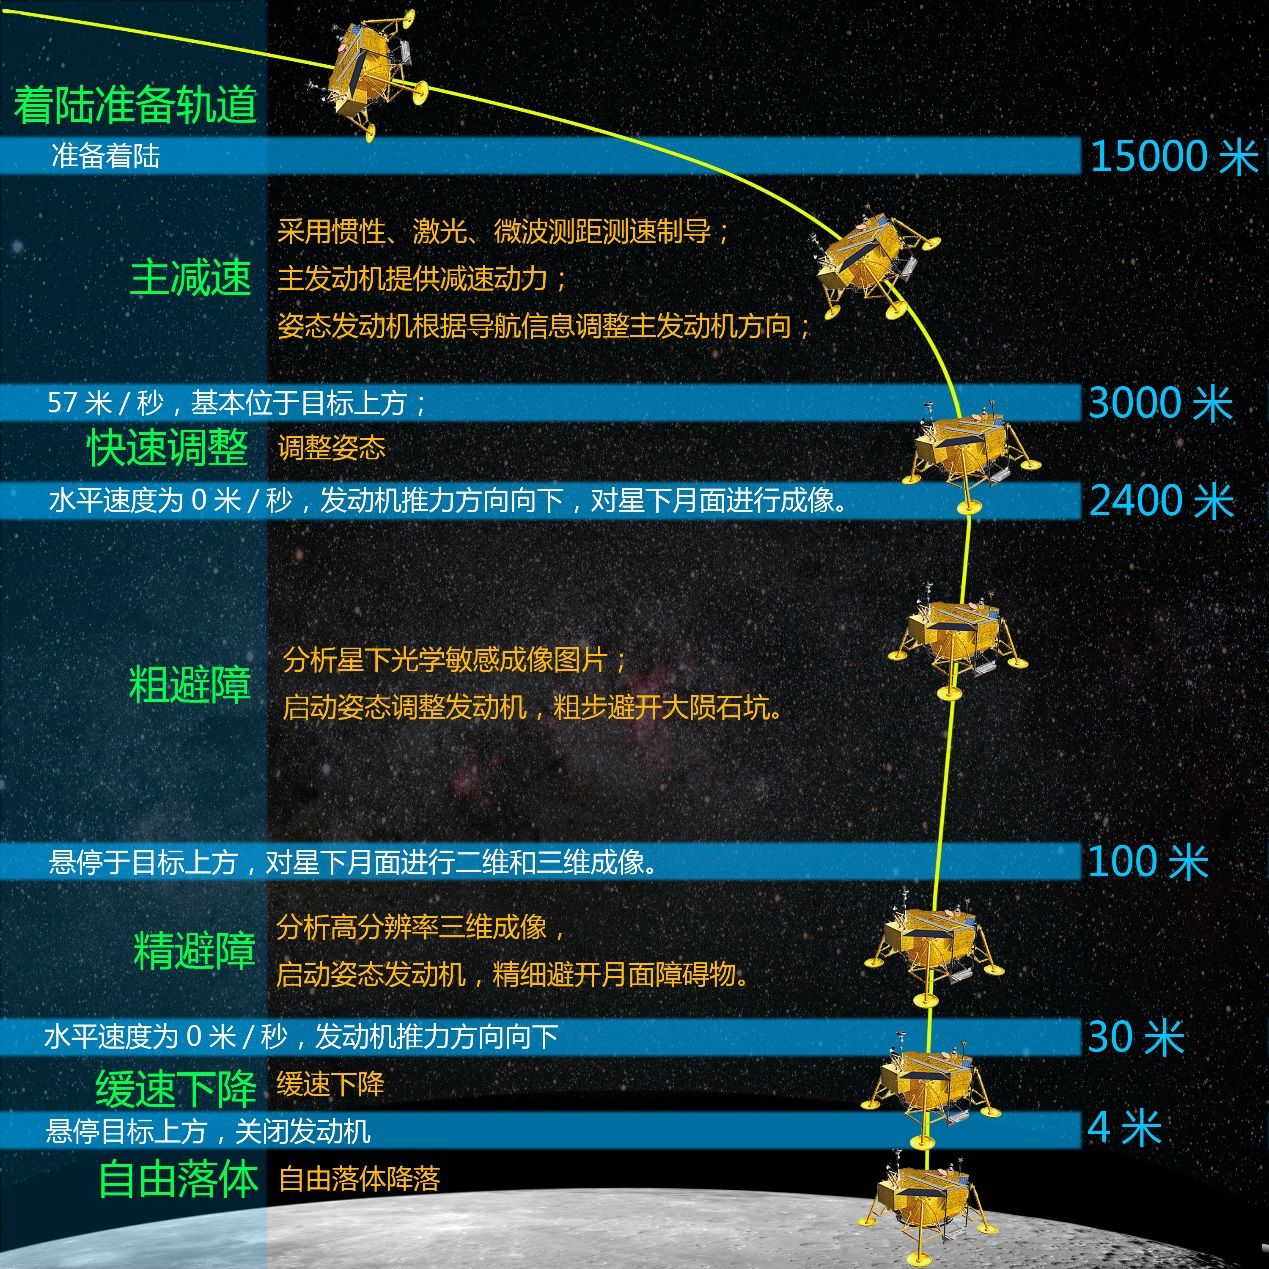
\includegraphics[width = 8cm]{images/Soft_landing_process.jpg}
            \caption{嫦娥三号软着陆过程示意图}
            \label{fig:嫦娥三号软着陆过程示意图}
            \end{figure}
            % \textcolor[rgb]{1 0 0}{todo:图片:附图4嫦娥三号软着陆过程示意图}
        \subsubsection{2.嫦娥三号软着陆过程分为6个阶段的要求}
            \par
            \textbf{(1)着陆准备轨道}:着陆准备轨道的近月点是15km,远月点是100km。近月点在月心坐标系的位置和软着陆轨道形态共同决定了着陆点的位置。
            \par
            \textbf{(2)主减速段}:主减速段的区间是距离月面15km到3km。该阶段的主要是减速,实现到距离月面3公里处嫦娥三号的速度降到$57m/s$。
            \par
            \textbf{(3)快速调整段}:快速调整段的主要是调整探测器姿态,需要从距离月面3km到 2.4km处将水平速度减为$0m/s$,即使主减速发动机的推力竖直向下,之后进入粗避障阶段。
            \par
            \textbf{(4)粗避障段}:粗避障段的范围是距离月面2.4km到100m区间,其主要是要求避开大的陨石坑,实现在设计着陆点上方100m处悬停,并初步确定落月地点。
            \par
            嫦娥三号在距离月面2.4km处对正下方月面$2300\times 2300m$的范围进行拍照,获得数字高程如附图(\ref{fig:距月面2400m处的数字高程图})所示(相关数据文件见附件3),并嫦娥三号在月面的垂直投影位于预定着陆区域的中心位置。
            \begin{figure}[H]
            \centering
            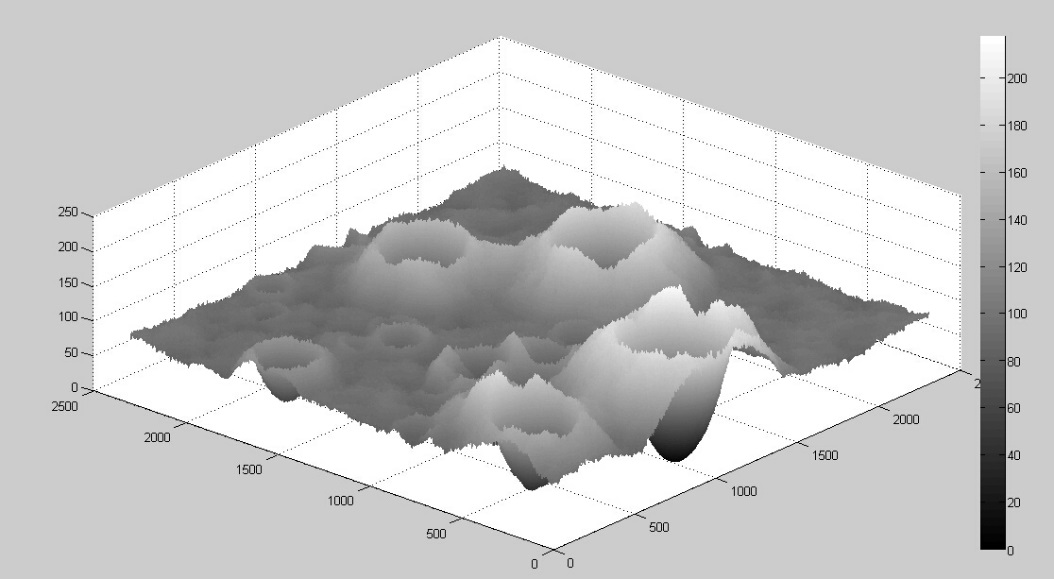
\includegraphics[height=4cm]{images/2400m_number.jpg}
            \caption{距月面2400m处的数字高程图}
            \label{fig:距月面2400m处的数字高程图}
            \end{figure}
            \par
            该高程图的水平分辨率是1m/像素,其数值的单位是1m。例如数字高程图中第1行第1列的数值是102,则表示着陆区域最左上角的高程是102米。
            \par
            \textbf{(5)精避障段}:精细避障段的区间是距离月面100m到30m。要求嫦娥三号悬停在距离月面100m处,对着陆点附近区域100m范围内拍摄图像,并获得三维数字高程图。分析三维数字高程图,避开较大的陨石坑,确定最佳着陆地点,实现在着陆点上方30m处水平方向速度为$0m/s$。附图(\ref{fig:距离月面100m处的数字高程图})是在距离月面100m处悬停拍摄到的数字高程图(相关数据文件见附件4)。
            \begin{figure}[H]
            \centering
            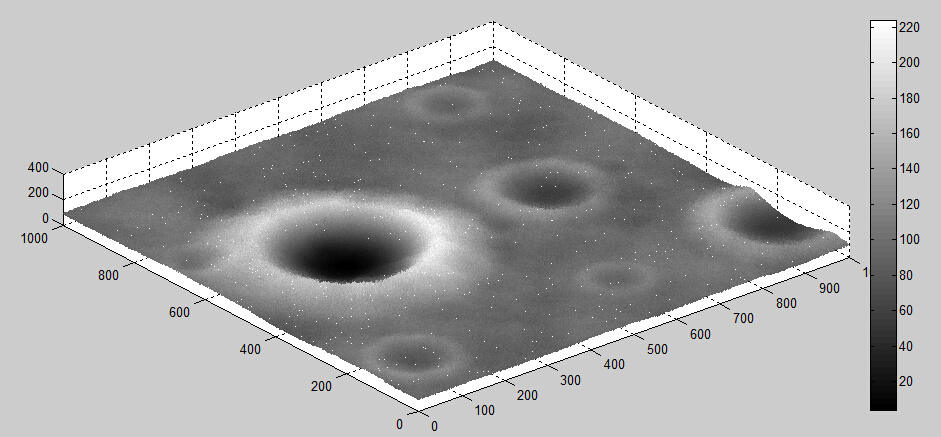
\includegraphics[height=4cm]{images/100m_number.jpg}
            \caption{距离月面100m处的数字高程图}
            \label{fig:距离月面100m处的数字高程图}
            \end{figure}
            \par
            该数字高程的水平分辨率为0.1m/像素,高度数值的单位是0.1m。
            \par
            \textbf{(6)缓速下降阶段}:缓速下降阶段的区间是距离月面30m到4m。该阶段的主要任务控制着陆器在距离月面4m处的速度为0m/s,即实现在距离月面4m处相对月面静止,之后关闭发动机,使嫦娥三号自由落体到精确有落月点。
            \par
            \textbf{注}:附件3和附件4中数字高程图对应的*.tif文件可以使用Matlab的“imread”命令打开,“imread”的具体使用方法见Matlab相关帮助。
    \subsection{附件3:距月面2400m处的数字高程图;}
            \begin{figure}[H]
            \centering
            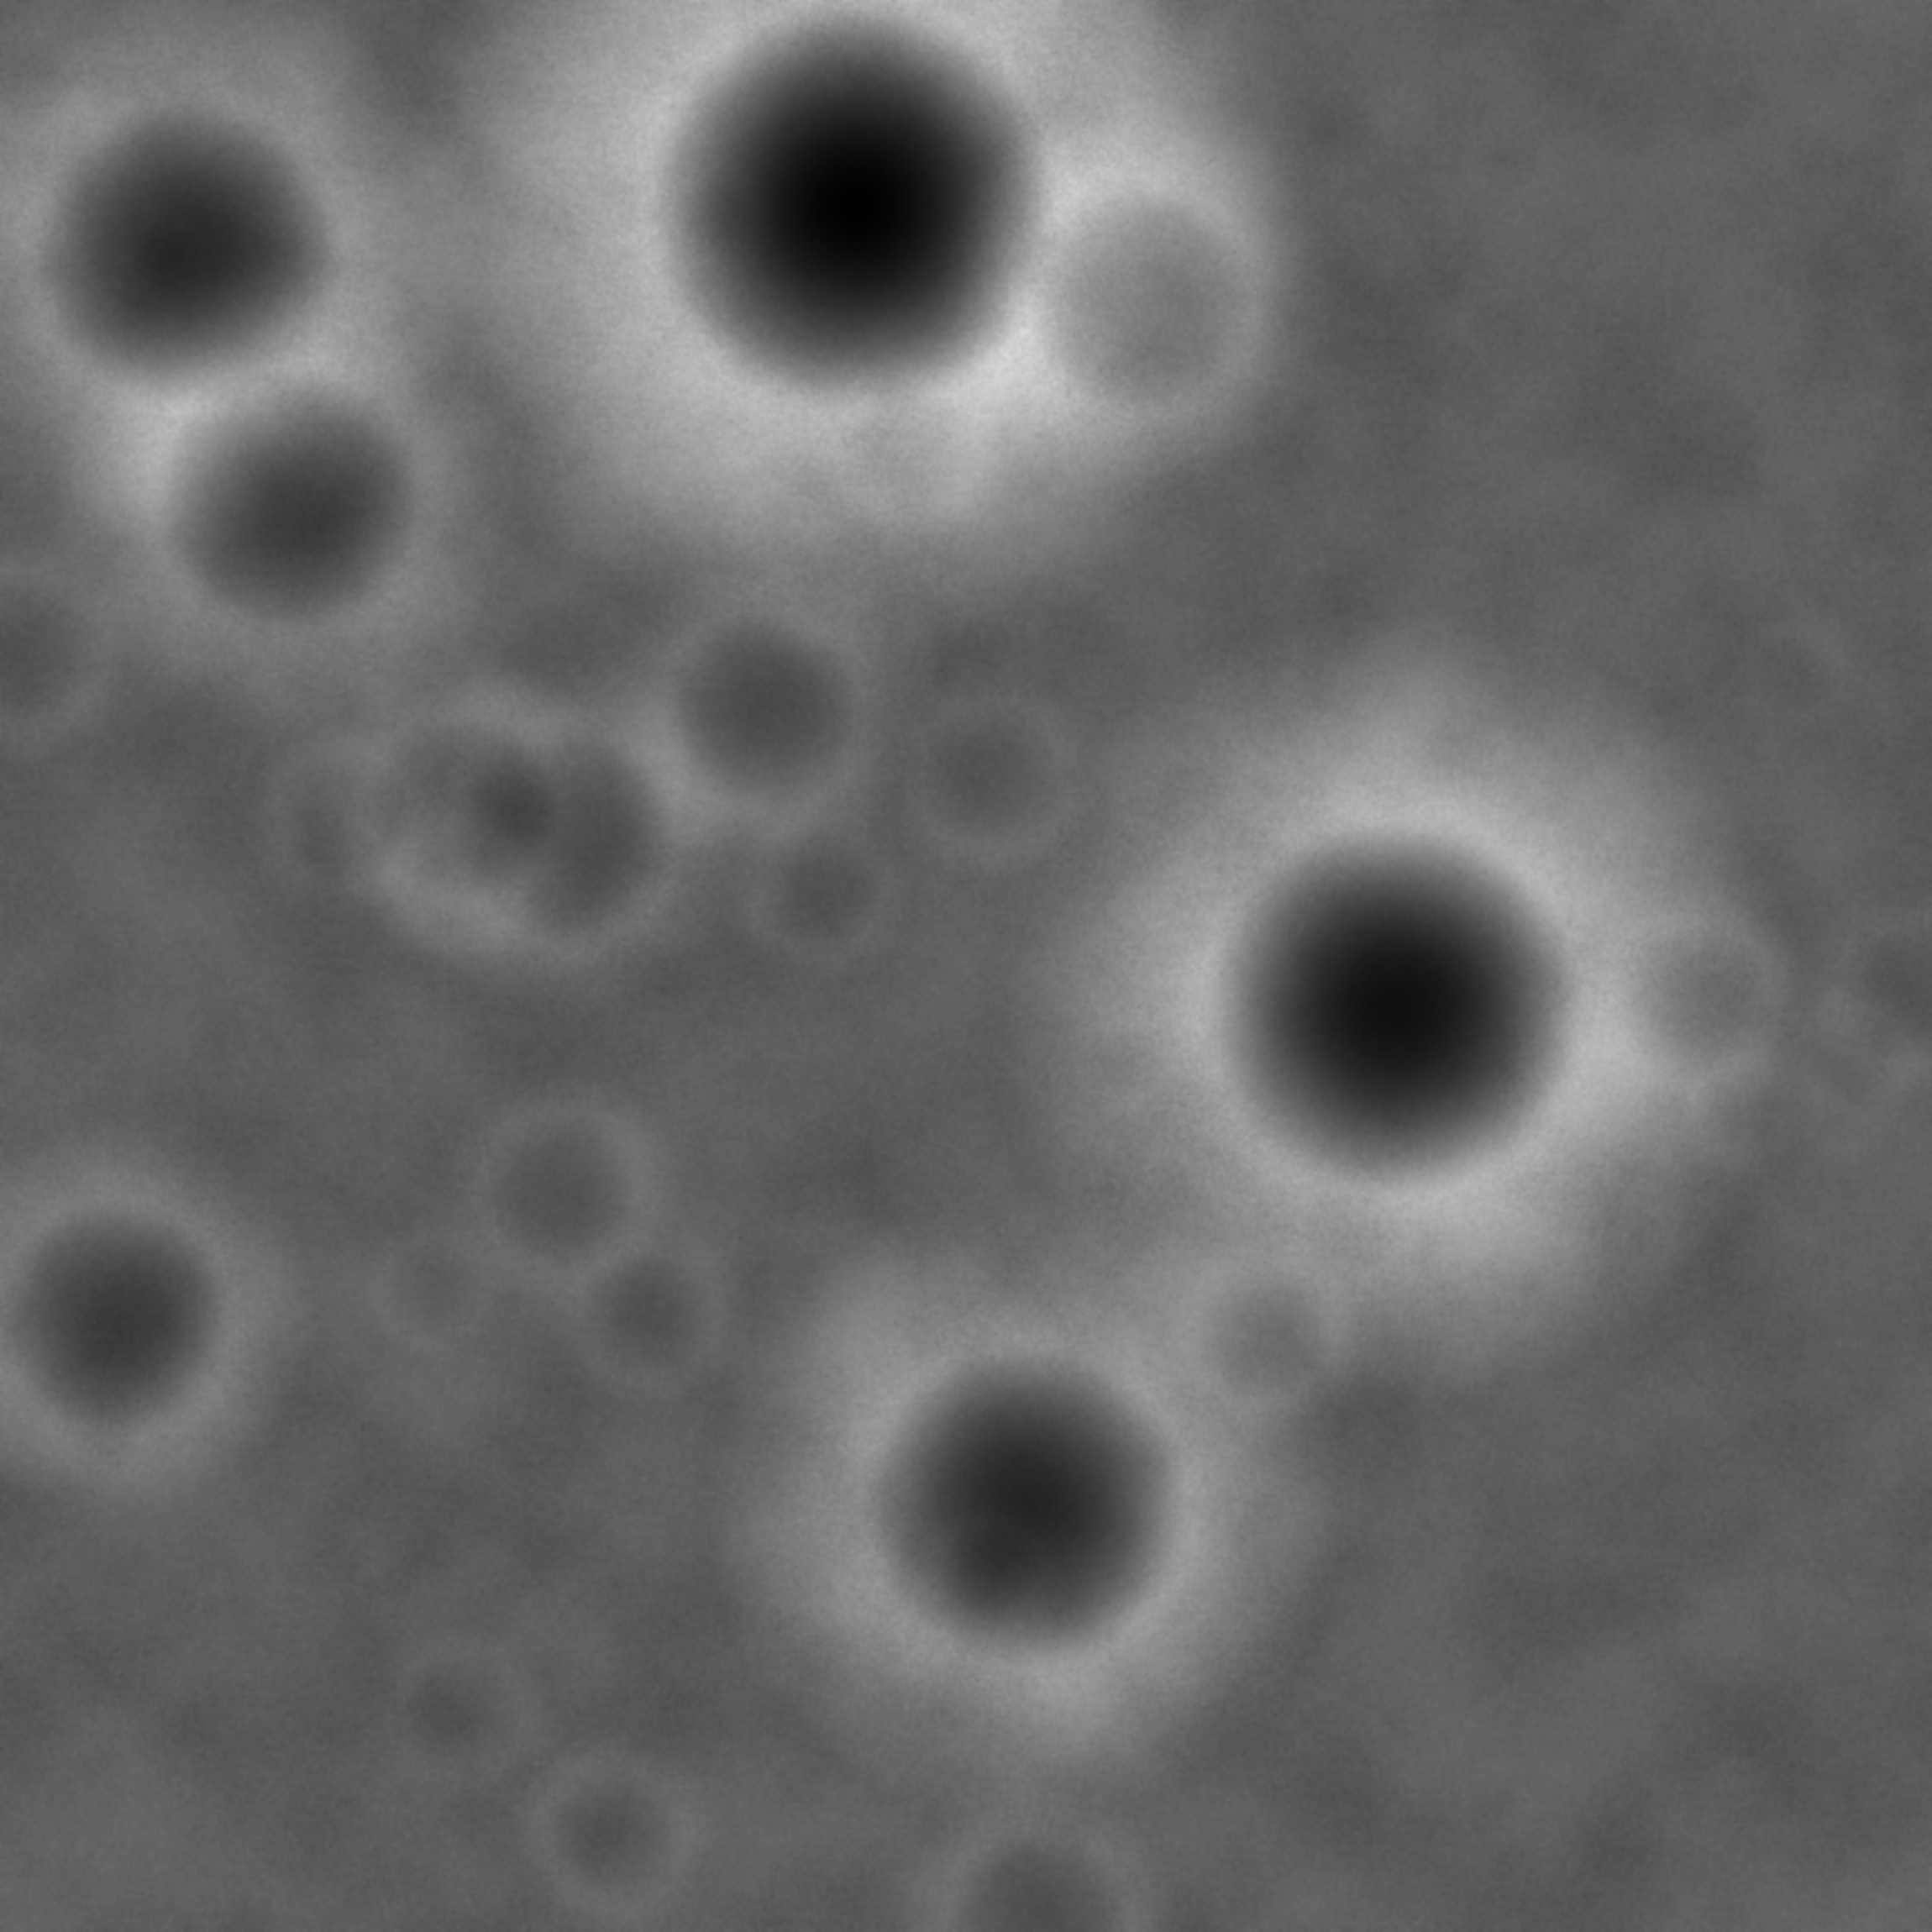
\includegraphics[height=6cm]{images/2400m_number2.png}
            \caption{距2400m处的数字高程图}
            \label{fig:距2400m处的数字高程图}
            \end{figure}
        % \textcolor[rgb]{1  0 0}{todo:图片:附件3 距2400m处的数字高程图}
    \subsection{附件4:距月面100m处的数字高程图。}
            \begin{figure}[H]
            \centering
            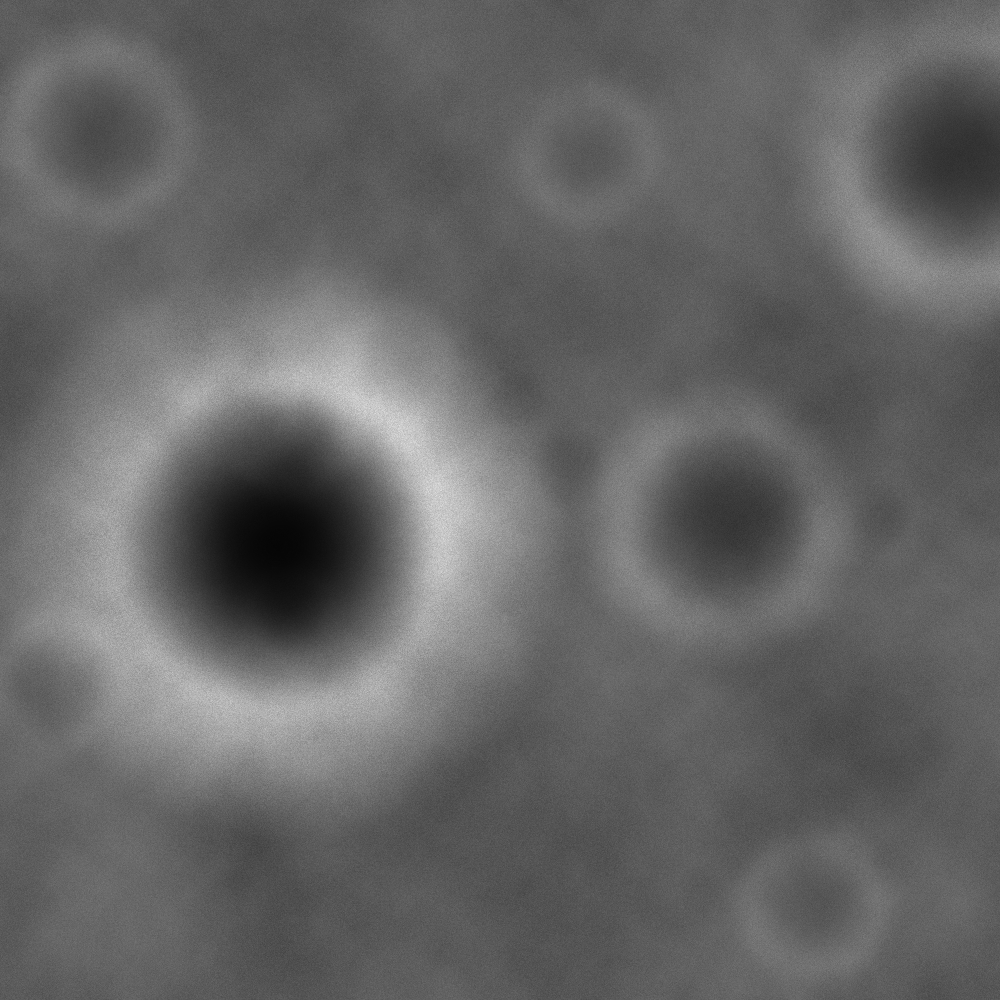
\includegraphics[width=6cm]{images/100m_number2.png}
            \caption{距月面100m处的数字高程图}
            \label{fig:距月面100m处的数字高程图}
            \end{figure}
\section{嫦娥3号软着陆的优化控制}
    \subsection{基础知识准备}
        \subsubsection{系统及最优控制基础知识}
            \par
            下面的内容介绍了一些系统和最优控制的基础知识。现代控制理论形成的主要标志是:1.Kalman滤波理论;2.Pontryayin极大值原理;3.Belman动态规划方法。主要分支有线性系统理论、最优控制理论、自适应控制、动态系统辨识、大系统理论等。
            \par
            状态:是一些变量的集合,它们是足以完全描述系统全部运动的最小变量集。
            \par
            完全描述:只要给定这组变量的某一初始时刻$t_0$的值,并且有输入控制函数$u(t)$,那么系统中的全部变量在$t \leqslant t_0$的值都唯一确定。
            \par
            状态向量:如果$n$个状态变量用$x_1(t),x_2(t),\dots,x_n(t)$表示,则
            \begin{align*}
            x(t) = [x_1(t),x_2(t),\dots,x_n(t)]^\mathrm{T}
            \end{align*}
            记为状态变量。
            \par
            状态方程:由系统的状态变量构成的一阶微分方程组称为状态方程。
            \par
            示例:考虑下面的例子,线性弹簧-质量-阻尼器构成的机械位移系统($k-m-f$)如图(\ref{fig:弹簧阻尼位移系统})所示
            \begin{figure}[H]
            \centering
            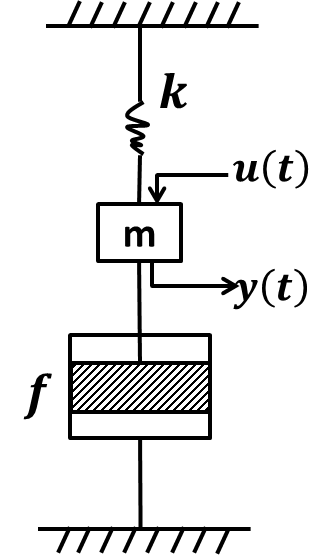
\includegraphics[height=4cm]{images/spring.jpg}
            \caption{弹簧阻尼位移系统}
            \label{fig:弹簧阻尼位移系统}
            \end{figure}
            如果输入量是外力$F(t)$,输出量是位移$y(t)$,则
            \begin{align*}
            m\frac{\mathrm{d}^2y}{\mathrm{d}t^2} + f\frac{\mathrm{d}y}{\mathrm{d}t} + ky =F(t)
            \end{align*}
            $y(t),\frac{\mathrm{d}y}{\mathrm{d}t}$就是足以完全描述系统运动的最小一组变量。输入量$u(t)= (F_t,\theta_t)$,输出量$y(t) = m_t$,状态量$x(t) = (v,r,w)$。
            \par
            上面介绍了系统的一些基本定义,下面我们介绍基于系统的最优控制问题,以及用变分法、P极大值原理、动态规划等技术求解系统的最优控制问题。常见的最优控制包括最短时、最少能耗及其组合优化问题。
            \par
            经典控制论中常用一个高阶微分方程来描述系统的运动规律,而现代控制论中采用是状态空间法,即为一组状态变量的一阶微分微分方程的形式作为系统的数学模型。这使得我们可以求解系统中许多量的值。MATLAB:控制系统工具箱Control System Toolbox、系统辨识工具箱System Idemtification Toolbox、鲁棒性控制工具箱Robust Control Toolbox、多变量频域设计工具箱Muli-Vanable Frequency Design Toolbox、最优化工具箱Ootimization Control toolbox以及Similink控制系统仿真环境。
            \par
            抽象系统方程为
            \begin{align*}
            \dot{x}(t) = F(x(t),u(t),t)
            \end{align*}
            其中:$x(t)$为$n$个状态变量$x_1,x_2,\dots,x_n$的向量形式;$u(t)$为控制输入$u_1,u_2,\dots,u_r$的向量形式;$F=(f_1,f_2,\dots,f_n)^\mathrm{T}$是一个函数标量。
            \par
            输出方程为
            \begin{align*}
            Y(t) = G(x(t),u(t),t)
            \end{align*}
            其中:$G=(g_1,g_2,\dots,g_m)^\mathrm{T}$是函数矢量。
            \par
            现代控制理论中,用系统状态方程和输出方程来描述系统的状态行为,状态方程和输出方程,合起来称为系统的状态表达式/动态方程。根据一阶微分方程$(F,G)$的形式,一般系统可分为:1.线性定常系统;2.线性不定常系统;3.非线性定常系统;4.非线性不定常系统。即
            \begin{align*}
            & \dot{x} = A x\\
            & \dot{x} = A(t)x\\
            & \dot{x} = Ax^2+x\\
            & \dot{x} = A(t)x^2+x
            \end{align*}
            对于一个系统的分析,一般有以下步骤:1.系统动态方程表达;2.系统状态方程的求解;3.系统稳定性及李雅普诺夫稳定;4.能控制和能观性;5.系统的最优控制。
            \par
            在最优控制过程中,我们不仅要给出系统的动态方程,而且还要注意系统变量的额约束。对系统状态$x(t)$而言,要考虑系统的始、终端条件。始终端约束条件即系统在时间$t_0$和$t_f$时,状态$x,x_f$应该满足一定的条件。端点条件一般有3种类型:1.固定端;2.自由端;3.可变端(灰色端)。
            \par
            固定端就是时间$t_0,t_f$固定,状态值$x_0,x_f$固定;自由端是指时间$t_0,t_f$固定,但端点状态$x_0,x_f$不变受任何限制的端点;可变端是指$t_0,t_f,x_0,x_f$都变的端点,但其一般应该满足某些条件,例如$N[x_f,t_f] = 0$,灰色端$\Delta_1 \leqslant x_f \leqslant \Delta_2$。
            \par
            对系统控制变量$u_t$而言,控制输入$u(t)$往往不能不受限制,因为其往往表示非常实际的物理量(例如:推理$F_t$,夹角$\theta_t$)。因此,实际中其约束一般表示$u_t$在某一范围内取值,如下表示
            \begin{align*}
            u_{min}  \leqslant u(t) \leqslant u_{max}
            \end{align*}
            由控制约束条件所规定的点集称为控制域,记为$ R_u$。
            \par
            凡在区间$[t_0,t_f]$内定义,且在$R_u$内取值的每一个控制函数$u_t$均称为容许控制,$u(t)\in R_u$。
            \par
            最优控制的目标泛函:系统的性能指标一般都是一个控制信号($\dot{m}(t)$函数)的函数,即泛函。对连续时间系统,目标泛函一般为
            \begin{align*}
            J = \Phi[x(t_f)] +\int_{t_0}^{t_f}L(x(t),u(t),t)\mathrm{d}t
            \end{align*}
            上述目标形式称为综合型/Bolza型。
            \par
            \begin{align*}
            J = \Phi[x(t_f)]
            \end{align*}
            称为终端型/Mayer型。
            \par
            \begin{align*}
            J = \int_{t_0}^{t_f} L[x(t),u(t),t]\mathrm{d}t
            \end{align*}
            称为积分型/Langrange型。其中:$L$为标量函数。最优控制问题即是在问题空间中,求解最优控制$u(t)^*$,使目标泛函$J$最优。
            \par
            解法:最优控制问题实际上就是微分代数混合优化问题,一般有两种求解方法:解析法和数值法。解析法又分为变分法和贝尔曼最佳原理的动态规划方法,但我们所建立的许多模型都相对复杂,解析法并不是非常适用,所以在书中大多数地方,我们都讨论问题的数值解法。下面,我们将简单介绍一下经典的最优控制解析方法:1.变分法;2.P极大值原理;3.动态规划。
        \subsubsection{变分法}
            \par
            考虑无约束情况下的极值问题。(1)一元函数极值:设$f(x)$为定义在$[a,b]$上的连续可微函数,且二阶可微。如果
            \begin{align*}
            \frac{\mathrm{d}y}{\mathrm{d}x}\Big|_{x=x_0} = f'(x)|_{x=x_0} = 0\\
            \frac{\mathrm{d}^2y}{\mathrm{d}x^2}\Big|_{x=x_0} = f''(x)|_{x=x_0} > 0
            \end{align*}
            则$f$在$x_0$处为极小值。
            \par
            (2)二元函数极值:设$f(x,y)$为定义在$D$上的连续可微函数,且二阶可微。如果
            \begin{align*}
            \left\{
            \begin{aligned}
            \frac{\partial f}{\partial x} \Big|_{x = x_0}\\
            \frac{\partial f}{\partial y} \Big|_{y = y_0}
            \end{aligned}
            \right.
            \end{align*}
            且$\frac{\partial ^2f}{\partial x^2}<0$,则$f$在点$(x_0,y_0)$处获得极小值。
            \par
            (3)多元极值:对一个$n$元函数$J = f(x)$,取极值的必要条件
            \begin{align*}
            \frac{\partial f}{\partial x} = 0
            \end{align*}
            取极小值的充分必要条件是
            \begin{align*}
            \frac{\partial ^2f}{\partial x^2} > 0
            \end{align*}
            其中:$\frac{\partial ^2f}{\partial x^2} = H$为Hessi矩阵,若Hessi矩阵为负定,则函数存在极大值。
            \par
            (4)泛函的定义:泛函可以简单理解为函数的函数。设对自变量$t$存在一类函数$\{x(t)\}$,如果$\forall x_t\in \phi $,有一个$J$值与之对应,则变量$J$称为依赖于函数$x(t)$的泛函数,简称泛函,如图(\ref{fig:泛函示意图})所示
            \begin{figure}[H]
            \centering
            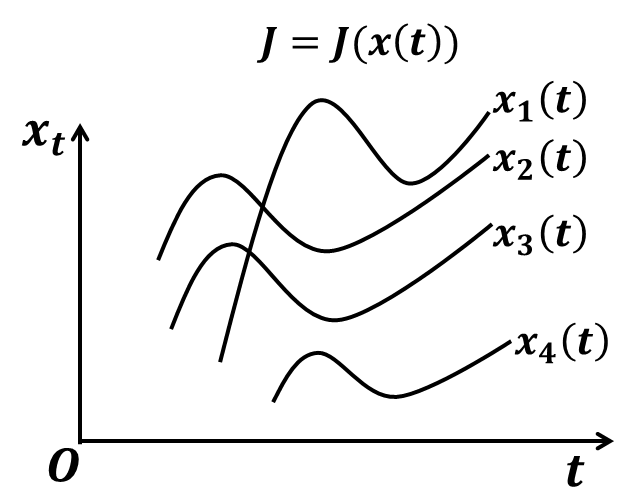
\includegraphics[height=4cm]{images/Functional_diagram.jpg}
            \caption{泛函示意图}
            \label{fig:泛函示意图}
            \end{figure}
            将$\{x_i(t)\}_{i=1}^4$带入某关系式,有$J = Af[x(t)]$。故称$J$为依赖$x(t)$的泛函,它是普通函数的一种扩充,函数$x(t)$称为$J$的宗基。当然,$\{x(t)\}$可以是一参数函数族:$x(t|\theta)$。
            \par
            由上述泛函定义可见,泛函是一标量,例如
            \begin{align*}
            J[x(t)] = \int_0^1x(t)\mathrm{d}t
            \end{align*}
            当$x(t) = \frac{1}{2}t$时,$J=1$;当$x(t) = \cos t$时,$J = \sin 1$。在最优控制中
            \begin{align*}
            J = \int_{t_0}^{t_f}L[x(t),u(t),t]\mathrm{d}t + \Delta
            \end{align*}
            $J$取决于$u(t),x(t)$,故$J$为泛函。
            \par
            在学习函数时,我们讨论了函数的连续性、函数导数和极值问题,那么,对于泛函,我们仍然讨论与之相似的问题。
            \par
            (5)泛函的连续性:称宗量$x(t)$的增量(两函数之差)为$x(t)$的变分
            \begin{align*}
            \delta x = x(t) - x_0(t)
            \end{align*}
            那么有
            \begin{align*}
            \delta\dot{x} = \frac{\mathrm{d}}{\mathrm{d}x} (\delta x)
            \end{align*}
            即导数的变分等价于变分的导数,且$\delta x$是变量$t$的函数$\delta x(t)$。
            \begin{definition}[泛函的连续性]
            如果对于$x(t)$的微小变化,有$J[x(t)]$的微小变化与之对应,则说$J[x(t)]$是连续的。对$\forall \epsilon >0$,$\exists \delta >0$,当
            \begin{align*}
            & |x(t) - x_0(t)| < \delta\\
            & | \dot{x}(t) - \dot{x}_0(t) |<\delta\\
            & \quad \vdots\\
            & | \dot{x}^k(t) - x_0^k(t) | < \delta
            \end{align*}
            时,有$|J[x(t)] - J[x_0(t)]  |<\epsilon$,则称$J[x(t)]$在$x_0(t)$处是$k$阶接近连续的。
            \end{definition}
            \par
            泛函的连续性如图(\ref{fig:泛函的连续性示意图})所示
            \begin{figure}[H]
            \centering
            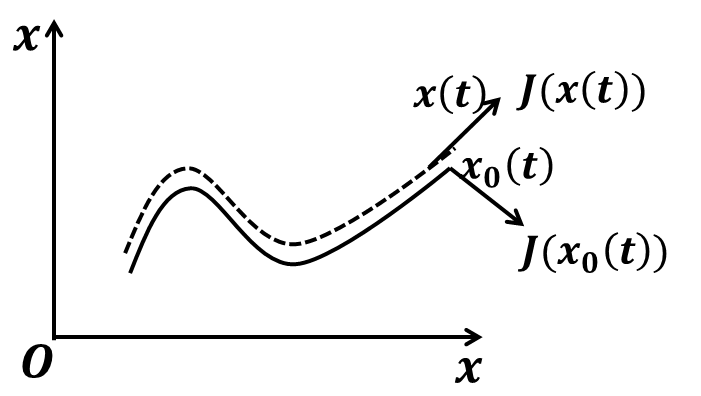
\includegraphics[height=4cm]{images/continuity_of_function_diagram.jpg}
            \caption{泛函的连续性示意图}
            \label{fig:泛函的连续性示意图}
            \end{figure}
            \par
            (6)泛函的变分:在函数中,微分是函数增量$\Delta y$对自变量$\Delta x$的线性部分。那么,在泛函中亦可将变分视为泛函增量$\Delta J$对宗量$x(t)$的线性部分,即当宗量$x(t)$有增量$\delta x(t)$时,泛函$J[x(t)]$的增量可以表示为
            \begin{align*}
            \Delta J = J[x(t) - \delta x(t)] - J[x(t)] = L[x(t),\delta x(t)]+r[x(t),\delta x(t)]
            \end{align*}
            其中:$L[x(t),\delta x(t)]$是泛函增量的线性主部分。故
            \begin{align*}
            \delta J = L[x(t),\delta x(t)]
            \end{align*}
            称为$J$的变分。
            \par
            泛函变分的求法:$J[x(t)]$的变分等于泛型$J[x(t)+\alpha \delta x(t)]$对$\alpha$的导数在$\alpha=0$时的值
            \begin{align*}
            \delta J = \frac{\partial }{\partial \alpha}J[x(t)+\alpha \delta x(t)]\big|_{\alpha=0} = L[x(t),\delta x(t)]
            \end{align*}
            \par
            (7)泛函极值:泛函极值的定义
            \begin{definition}[泛函极值]
            如果$J$在任意一点与$x_0(t)$接近的曲线$x(t)$上的值不小于$J[x_0(t)]$,即
            \begin{align*}
            J[x(t)] - J[x_0(t)] \geqslant 0
            \end{align*}
            则$J$在$x_0(t)$上达到极小值。
            \end{definition}
            \par
            泛函极值的必要条件(无约束):若$J$在$x_0(t)$处达到极小值,则在$x(t) = x_0(t)$上有
            \begin{align*}
            \delta J = 0
            \end{align*}
            上述欧拉方程是泛函极值的必要条件而非充分。
            \par
            固定端点的泛函极值问题:已知宗量$x(t)$在$t_0$时为$x_0$,在$t_f$时为$x_f$,则使积分型性能指标函数
            \begin{align*}
            J = \int_{t_0}^{t_f}L[x(t),\dot{x}(t),t]\mathrm{d}t
            \end{align*}
            取极值的必要条件为$x^*(t)$满足下面的欧拉方程
            \begin{align*}
            \frac{\partial L}{\partial x} - \frac{\mathrm{d} }{\partial t}\frac{\partial L}{\partial \dot{x}} = 0
            \end{align*}
            其中:$L$及$x(t)$在$[t_0,t_f]$上至少两次连续可微。
            \par
            将上述结论推广至多变量系统
            \begin{align*}
            \left\{
            \begin{aligned}
            & J = \int_{t_0}^{t_f}L[x(t),\dot{x}(t),t]\mathrm{d}t\\
            & x(t_0) = x_0\\
            & x(t_f) = x_f
            \end{aligned}
            \right.
            \end{align*}
            $J$极值存在的必要条件为
            \begin{align*}
            \frac{\partial L}{\partial x} - \frac{\mathrm{d} }{\partial t}\frac{\partial L}{\partial \dot{x}} = 0
            \end{align*}
            及横截条件方程
            \begin{align*}
            \left( \frac{\partial L}{\partial \dot{x}} \right) ^\mathrm{T}\Big|_{t = t_f}\delta x(t_f) - \left( \frac{\partial L}{\partial \dot{x}} \right) ^\mathrm{T}\Big|_{t=t_0}\delta x(t_0) = 0
            \end{align*}
            其中:
            \begin{align*}
            \frac{\partial L}{\partial x} = \left[\frac{\partial L}{\partial x_1},\frac{\partial L}{\partial x_2} ,\dots, \frac{\partial L}{\partial x_n}\right]^\mathrm{T}\\
            \frac{\partial L}{\partial \dot{x}} = \left[\frac{\partial L}{\partial \dot{x}_1},\frac{\partial L}{\partial \dot{x}_2} ,\dots, \frac{\partial L}{\partial \dot{x}_n}\right]^\mathrm{T}
            \end{align*}
            \par
            示例:求泛函
            \begin{align*}
            \left\{
            \begin{aligned}
            & J(x_1,x_2) = \int_{0}^{\frac{\pi}{2}} [2x,x_2+\dot{x}_1^2+\dot{x}_2^2]\mathrm{d}t\\
            & x_1(0) = 0,x_2({\pi}/{2}) = 1\\
            & x_2(0) = 0,x_2({\pi}/{2})=1
            \end{aligned}\right.
            \end{align*}
            下的极值。求解程序如下
            \begin{lstlisting}[language = Matlab]
            [x1,x2] = dsolve('D2x1-x2=0','D2x2-x1=0',...
            'x1(0)=0','x1(pi/2)=1','x2(0)=0','x2(pi/2)=-1','t')
            \end{lstlisting}
            \par
            可变端点极值问题的必要条件:设宗量$x(t)$自一给定点$(t_0,x_0)$达到给定$x(t_f) = \varphi(t_f)$上某一点$[t_f,\varphi(t_f)]$,使
            \begin{align*}
            J = \int_{t_0}^{t_f} L[x(t),\dot{x}(t),t]\mathrm{d}t
            \end{align*}
            取极值的必要条件为$x^*(t)$满足如下欧拉方程
            \begin{align*}
            \frac{\partial L}{\partial x} - \frac{\mathrm{d} }{\partial t}\frac{\partial L}{\partial \dot{x}} = 0
            \end{align*}
            及
            \begin{align*}
            & x(t_0) = x_0\\
            & \left\{L[x,\dot{x},t]+(\dot{\varphi}-\dot{x})^\mathrm{T}\frac{\partial L}{\partial \dot{x}}  \right\}\Big|_{t=t_f}=0\\
            & x(t_f) = \varphi(t_f)
            \end{align*}
            其中:$x(t)$连续两阶可导;$L$至少两次连续可微;$\varphi(t)$有连续一次导数。可变端点极值问题示意图如图(\ref{fig:可变端点极值问题示意图})所示
            \begin{figure}[H]
            \centering
            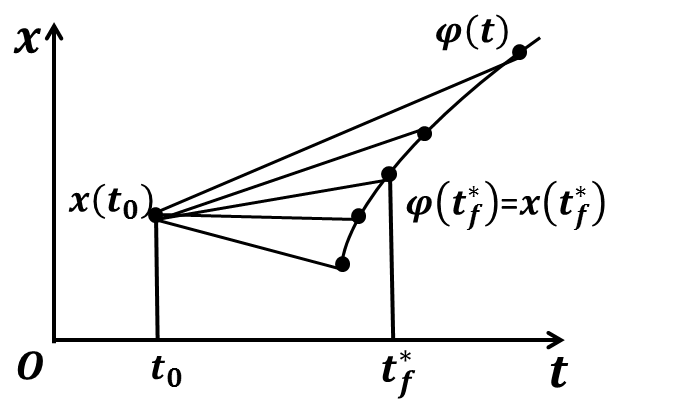
\includegraphics[height=4cm]{images/Variable_Extreme_Extreme_Value_Problem.jpg}
            \caption{可变端点极值问题示意图}
            \label{fig:可变端点极值问题示意图}
            \end{figure}
        \subsubsection{变分法求解最优控制问题}
            \par
            前面导出了极值曲线$x^*(t)$存在的必要条件-欧拉方程和横截条件($x(t)$无约束),而在最优控制中,$x(t)$除了要满足限制条件外,还应该满足某些系统动态方程,它可以看成一种等式约束,可采用拉格朗日乘子法进行处理。将等式约束下对$J$的优化转化为无约束条件下就Hamilton的极值问题。它只适用于控制变量无约束的情况。
            \begin{align*}
            & \min_{u(t)} \ J = \int_{t_0}^{t_f}L[x(t),u(t),t]\mathrm{d}t\\
            & s.t.\left\{
            \begin{aligned}
            & \dot{x}(t) = f[x(t),u(t),t]\\
            & x(t_0) = x_0\\
            & x(t_f) = x_f
            \end{aligned}
            \right.
            \end{align*}
            \ding{172}固定端点的控制问题\label{固定端点的控制问题};\ding{173}可变端点的控制\label{可变端点的控制}($t_f$固定,$x(t_f)$自由;$t_f$固定,$x(t_f)$有约束;$t_f$可变,$x(t_f)$有约束)。对问题\ding{172}(\ref{固定端点的控制问题}),引入拉格朗日乘子$\lambda(t) = [\lambda_1(t),\lambda_2(t),\dots,\lambda_n(t)]^\mathrm{T}$,构建哈密顿标量函数
            \begin{align*}
            H[x(t),u(t),\lambda(t),t]= L[x(t),u(t),t]+\lambda^\mathrm{T}(t)f[x(t),u(t),t]
            \end{align*}
            则上述优化问题变为
            \begin{align*}
            J = \int_{t_0}^{t_f}  H[x(t),u(t),\lambda(t),t] - \lambda^\mathrm{T}x(t)\mathrm{d}t
            \end{align*}
            由欧拉方程得
            \begin{align*}
            & \frac{\partial [H-\lambda^\mathrm{T}\dot{x}]}{\partial x}-\frac{\mathrm{d}}{\mathrm{d}t}\frac{\partial [H - \lambda^\mathrm{T}\dot{x}]}{\partial \dot{x}} = 0\\
            \Rightarrow{} & \dot{\lambda} = -\frac{\partial H}{\partial x} \quad \text{伴随方程}\\
            & \frac{\partial [H-\lambda^\mathrm{T}\dot{x}]}{\partial u}-\frac{\mathrm{d}}{\mathrm{d}t}\frac{\partial [H - \lambda^\mathrm{T}\dot{x}]}{\partial \dot{u}} = 0\\
            \Rightarrow{} &\frac{\partial H}{\partial u} = 0 \quad \text{控制方程}\\
            & \frac{\partial [H-\lambda^\mathrm{T}\dot{x}]}{\partial \lambda}-\frac{\mathrm{d}}{\mathrm{d}t}\frac{\partial [H - \lambda^\mathrm{T}\dot{x}]}{\partial \dot{\lambda}} = 0\\
            \Rightarrow{} & \dot{x} = -\frac{\partial H}{\partial \lambda} = f(x,u,t) \quad \text{状态方程}\\
            \end{align*}
            及边界条件(横截条件)
            \begin{align*}
            & \frac{\partial [H-\lambda^\mathrm{T}\dot{x}]}{\partial \dot{x}}\Big|_{t=t_f} = 0\\
            \Rightarrow {} & \lambda(t_f) = 0
            \end{align*}
            状态方程与伴随方程合称为正则方程。
            \par
            求解过程:$\frac{\partial H}{\partial u} = 0$可求得最优控制$u^*$与$x$及$\lambda$的函数关系式,然后将其带入正则方程组中消去$u^*$,解两点边值问题
            \begin{align*}
            \left\{
            \begin{aligned}
            & \dot{x} = f(x,u(x,\lambda),t),\ x(t_0) =x_0\\
            & \dot{\lambda} = -\frac{\partial H}{\partial x}, \ x(t_f) = x_f
            \end{aligned}
            \right.
            \end{align*}
            可求得$x^*(t),\lambda^*(t)$,再将 $x^*,\lambda^*$带入$u(x^*,\lambda^*)$可得$u^*$的具体情况。另外,对$H$函数有
            \begin{align*}
            \frac{\mathrm{d}H}{\mathrm{d}t} & = \frac{\partial H}{\partial t} + \left( \frac{\partial H}{\partial u} \right)^{\mathrm{T}}\dot{u} + \left( \frac{\partial H}{\partial x} \right)^\mathrm{T}\dot{x} + \left( \frac{\partial H}{\partial \lambda} \right)^\mathrm{T}\dot{\lambda}\\
            & =\frac{\partial H}{\partial t}+ \left( \frac{\partial H}{\partial u} \right) ^\mathrm{T}\dot{u}+\left( \frac{\partial H}{\partial x}+\dot{\lambda} \right) ^\mathrm{T}f
            \end{align*}
            当$\frac{\partial H}{\partial u}\frac{\partial H}{\partial x} = \lambda,\frac{\partial u}{\partial \lambda} = 0$时,$\frac{\mathrm{d}H}{\mathrm{d}t} = \frac{\partial H}{\partial t}$,即沿最优曲线,$H$对$t$的导数等于对时间的偏导数。注:上述欧拉方程式取极值的必要条件。
            \par
            下面,分析终端自由的情况\ding{173}(\ref{可变端点的控制}):
            \begin{align*}
            &J = \Phi[x(t_f),t_f]+\int_{t_0}^{t_f}L(x,u,t)\mathrm{d}t\\
            &s.t.\left\{
            \begin{aligned}
            &\dot{x} = f(x,u,t)\\
            &t_0,x_0\text{固定}
            \end{aligned}
            \right.
            \end{align*}
            求$t_f,x_f$自由时的最优控制$u^*$及最优轨线$x^*$。
            \par
            (1)构建$H$函数
            \begin{align*}
            H(x,u,\lambda,t) = L(x,u,t)+\lambda^\mathrm{T}f(x,u,t)
            \end{align*}
            \par
            (2)增广泛函$J'$
            \begin{align*}
            J'= \Phi[x(t_f),t_f]+\int_{t_0}^{t_f}[H - \lambda^\mathrm{T}x]\mathrm{d}t
            \end{align*}
            $J'$的一次变分为
            \begin{align*}
            \delta J' = \left( \frac{\partial \Phi}{\partial x(t_f)} \right)^\mathrm{T} \delta x(t_f) + \left( \frac{\partial \Phi}{\partial x(t_f)} \right)^\mathrm{T} \frac{\partial x(t_f)}{\partial t_f}\delta t_f+ \frac{\partial \Phi}{\partial t_f}\delta t_f+ [H-\lambda^\mathrm{T}\dot{x}]_{t_f} \delta t_f + \delta J_0
            \end{align*}
            其中:$\delta J_0 = \delta J_0[x,\dot{x},\lambda,u] = \delta \int_{t_0}^{t_f}[H-\lambda^\mathrm{T}\dot{x}]\mathrm{d}t$。
            \par
            泛函$J'$极值存在的必要条件是:$\delta J' = 0$。对固定时间$t_0,t_f$的变分,$\delta (t_0) = 0$
            \begin{align*}
            \delta J_0 &= \int_{t_0}^{t_f} \left[\frac{\partial \bar{H}}{\partial x} - \frac{\mathrm{d}}{\mathrm{d}t}\frac{\partial \bar{H}}{\partial \dot{x}}\right]^\mathrm{T}\delta x\mathrm{d}t +\int_{t_0}^{t_f} \left( \frac{\partial \bar{H}}{\partial u} \right) ^\mathrm{T}\delta u\mathrm{d}t\\
            &\quad +\int_{t_0}^{t_f} \left( \frac{\partial \bar{H}}{\partial \lambda} \right) ^\mathrm{T}\delta \lambda \mathrm{d}t+ \left( \frac{\partial \bar{H}}{\partial \dot{x}} \right)^\mathrm{T} \delta x\Big|_{t_0}^{t_f}
            \end{align*}
            其中:$\bar{H} = H - \lambda ^\mathrm{T}x$。将$\delta J_0$带入$\delta J'$,且令$\delta J'=0$,有
            \begin{align*}
            & \left.
            \begin{aligned}
            \dot{\lambda} = -\frac{\partial H}{\partial x}\\
            \dot{x} = -\frac{\partial H}{\partial \lambda}
            \end{aligned}
            \right\}
            \quad \text{正则方程}\\
            & \frac{\partial H}{\partial u} = 0\quad \text{控制方程}
            \end{align*}
            边界条件/横截条件
            \begin{align*}
            \left\{
            \begin{aligned}
            & \lambda(t_f) = \frac{\partial \Phi}{\partial x}\Big|_{t=t_f}\\
            & x(t_0) = x_0\\
            & H[x(t_f),u(t_f),t_f] = -\frac{\partial \Phi}{\partial t_f}
            \end{aligned}
            \right.
            \end{align*}
            \par
            \ding{172}终端$t_f$固定,$x(t_f)$自由时
            \begin{align*}
            \left\{
            \begin{aligned}
            & x(t_f) = \frac{\partial \Phi}{\partial x}\Big|_{t=t_f}\\
            & x(t_0) = x_0
            \end{aligned}
            \right.
            \end{align*}
            \par
            \ding{173}终端$t_f$固定,$x(t_f)$有约束:$N_1(x(t_f),t_f) = 0$,其中:$N_1 = [N_{11},N_{12},\dots,N_{1m}]^\mathrm{T}$
            \begin{align*}
            \left\{
            \begin{aligned}
            & \lambda(t_f) = \left[ \frac{\partial \Phi}{\partial x}+\left( \frac{\partial N_1^\mathrm{T}}{\partial x} \right)v  \right]\Big|_{t=t_f}\\
            & x(t_0) = x_0\\
            & N_1(x(t_f),t_f) = 0
            \end{aligned}
            \right.
            \end{align*}
            \par
            \ding{174}$t_f$可变,$x(t_f)$有约束:$N_1(x(t_f),t_f) = 0$
            \begin{align*}
            \left\{
            \begin{aligned}
            & \lambda(t_f) = \left[ \frac{\partial \Phi}{\partial x}+\left( \frac{\partial N_1^\mathrm{T}}{\partial x} \right)v  \right]\Big|_{t=t_f}\\
            & \left[ H+\frac{\partial \Phi}{\partial t}+v^\mathrm{T}\frac{\partial N_1}{\partial t}  \right]\Big|_{t=t_f} = 0\\
            & x(t_0) = x_0\\
            & N_1(x(t_f),t_f) = 0
            \end{aligned}
            \right.
            \end{align*}
            \par
            \ding{175}当$t_f,x(t_f)$稳定时
            \begin{align*}
            \mathrm{d}x(t_f) & = x(t_f+\delta t_f) + \delta x(t_f+\delta t_f) - x(t_f)\\
            & \delta x(t_f)+\dot{x}(t_f)\delta t_f
            \end{align*}
            \par
            \ding{176}当$x_f$固定,$t_f$自由时
            \begin{align*}
            \mathrm{d}x(t_f) = 0= \delta x(t_f)+\dot{x}\delta t_f
            \end{align*}
        \subsubsection{极大(小)值原理求解最优控制问题}
            \par
            上面介绍的变分法用于求解$u(t)$无约束的情况,而在实际过程中$u(t)$往往具有实际的物理意义,因此$u(t)$一般有约束,例如
            \begin{align*}
            A \leqslant u(t) \leqslant B
            \end{align*}
            设$R=\{u(t)|\forall t\in [t_0,t_f],A \leqslant u(t) \leqslant B\}$为函数空间。P极大值原理用于求解$u(t)$有约束的情况
            \begin{align*}
            \min_{u(t)} \ J = \Phi[x(t_f),t_f]+\int_{t_0}^{t_f} L[x(t),u(t),t]\mathrm{d}t\\
            s.t.\left\{
            \begin{aligned}
            x(t_0) = x_0\\
            \dot{x} = f(x(t),u(t),t)\\
            N_1[x(t_f),t_f] = 0\\
            g[x(t),u(t),t] \geqslant 0
            \end{aligned}
            \right.
            \end{align*}
            \par
            如何处理上面的$g \geqslant 0$?要是能将$g$变为等式约束就好了,我们仿照线性规划,引入人工变量$z,w$
            \begin{align*}
            (\dot{z})^2 = g[x,u,t] ,\quad z(t_0) = 0\\
            \dot{w} = u(t),\quad w(t_0)=0
            \end{align*}
            无论$\dot{z}$是正还是负,$(\dot{z})^2$恒非负。如$u(t)$是分段连续函数免责$w(t)$是分段光滑连续函数。如此,将$g \leqslant 0$转化为$(\dot{z})^2 =g[x(t),\dot{w}(t),t] $等式约束,继而可以引入拉格朗日乘子,构建$H$函数进行求解。
            \par
            实现最优控制的必要条件是:\\
            (1)$u^*,x^*,\lambda^*$满足下面条件
            \begin{align*}
            \dot{x} = \frac{\partial H}{\partial \lambda}\\
            \dot{\lambda} = -\frac{\partial H}{\partial x}
            \end{align*}
            其中:$H = L+\lambda^\mathrm{T}f$。\\
            (2)
            \begin{align*}
            H[x^*,u^*,\lambda^*,t] = \min_{u(t)\in R}H[x^*,u,\lambda^*,t]
            \end{align*}
            (3)端点边界条件与终端横截条件
            \begin{align*}
            & x(t_0) = x_0\\
            & N[x(t_f),t_f] = 0\\
            & \lambda_f = \left[ \frac{\partial \Phi}{\partial x}+ \left( \frac{\partial H_1}{\partial x} \right)^\mathrm{T}v  \right]\Big|_{t=t_f}
            \end{align*}
            (4)终端$t_f$可变时
            \begin{align*}
            \left[ H+\frac{\partial\Phi}{\partial t} +v^\mathrm{T}\frac{\partial N_1}{\partial t}\right]\Big|_{t = t_f} = 0
            \end{align*}
            \par
            最小时间控制
            \begin{align*}
            J = t_f\quad \text{砰-砰}
            \end{align*}
            最小能量控制
            \begin{align*}
            J = \int_{t_0}^{t_f}|u(t)|\mathrm{d}t \quad \text{砰-零-砰}
            \end{align*}
            最小时间能量综合控制
            \begin{align*}
            J = \int_{t_0}^{t_f} \rho+|u(t)| \mathrm{d}t\quad \text{砰-零-砰}
            \end{align*}
            其中:$\rho$为权重。
        \subsubsection{最优控制问题的数学提法}
            \par
            用极大值原理结合非线性规划来解决软着陆最小消耗问题,具有算法简单、原理可靠的特点,但其只能使发动机推力$F$为常量,且由于末端时刻未定,导致迭代次数较大。此外,还需要猜测无物理意义的协变量状态的初始值,这使系统很敏感。用“协状态-控制”变换可以从一定程度上减弱这种对初值的依赖性。为了避免上述缺点,下面引入参数化控制的方法,该方法是K.L.Teo和H.E.Jlee等人提出,主要思想是用若干个分段常值函数逼近最优解。
            \par
            (1)设控制系统的运动遵从抽象微分方程
            \begin{align*}
            \dot{x} = f(x(t),u(t),t) \quad t\in J
            \end{align*}
            其中:$f\in[X\times U\times J;Y]$;$J$为$[0,\infty)$中的某个连续闭子集,称为系统的时间域;$X$为Banach空间/拓扑线性空间,称为系统的相空间或状态空间;$U$为拓扑空间,称为系统的控制域;$t$为时间变量;$x$为状态变量;$u$为控制变量;$x$的具体情况为状态轨线,是时间$t$的函数,其图形是$J\times X$中的点集;相空间$X$中确定的点集$\{x(t)|t\in J\}$称为系统的一条相轨线,与$t$无关。
            \par
            (2)控制函数$u$的限制。例如要求$u(\cdot)$为简单函数、可测函数、连续函数、分段函数、分段可微等,即
            \begin{align*}
            \{u\} = \mathcal{U}\subset [J;U]
            \end{align*}
            \par
            (3)端点条件。有$t_0 = \int J,t_f = \sup J$,对于某个给定的点集$M=  M_0\times M_1 \subset Y\times X$
            \begin{align*}
            x(t_0) \in M_0\\
            x(t_f)\in M_1
            \end{align*}
            当$M_1=X$时,称为终端自由;当$t_f=\sup J<\infty$时,称终端时间$tf$固定。在许多控制问题中,控制系统的状态空间$X$是某个广义函数空间或抽象的向量值函数空间。
            \par
            假设一个控制系统的状态方程、控制域$U$、控制函数类$\mathcal{U}$以及约束条件均已给出,且相应的容许控制类$\mathcal{U}_{ad} \neq 0$。记全体容许对所构成的集合为$A_{ad}$,任一映射$J\in [A_{sd};R]$称为该控制系统的一个指标泛函。
            \par
            对于给定的指标泛函$J$,寻找适当的$(x,u)^*\in A_{ad}$,使得
            \begin{align*}
            J(x,u)^* = J^* = \inf\{J(x,u)|(x,u)^*\in A_{ad}\}
            \end{align*}
            如果这样的容许对$(x,u)^*$存在,则称该最优控制问题有解。$(x,u)^*$为最有对,$u^*$为最优控制,$x^*$为最优轨线。
            \par
            给出非线性标量型的最优化问题
            \begin{align*}
            & J = \phi_0[x(t_f|u)]+\int_{t_0}^{t_f}L_0[x(t|u),u(t),t]\mathrm{d}t\\
            & s.t.\quad g_i(u) = \phi_i[x(t_f|u)]+\int_{t_0}^{t_f}L_i[x(t|u),u(t),t] \mathrm{d}t \geqslant 0
            \end{align*}
            其中:$Q_i,L_i(i=1,2,\dots,N)$实值向量函数;$f:[0,t_f]\times R^{n_s}\times R^{n_c}\to R^{n_s}$;$\phi_i:R^{n_s}\to R,i=0,1,\dots,N$,$L_i = [0,t_f] \times R^{n_c}\times R^{n_c}\to R,i=0,1,\dots,N$。
            \par
            $\exists k$,$\forall (t,x,u)\in [0,t_f]\times R^{N_S}\times V$,均有$|f(t,u,x)| \leqslant k(1+|x|)$。其中:$V\in R^{n_c}$是$R_{n_c}$中任意紧致闭子集。泛函$f$和$L_i,i=0,1,\dots,N$,关于$x$和$u$的偏导数在$[t_0,t_f]$内均为分段连续函数。$\forall i,\phi_i$对$x,u$是连续可微的。
            \par
            参数化最优控制器设计。首先,选取一组满足$\{t_k^p\}_{k=0}^{n_p}$
            \begin{align*}
            t_0 = t_0^p<t_1^p<t_2^p <\dots<t_{n_p}^p = t_f
            \end{align*}
            和一组参数$\sigma_k^p,k=1,2,\dots,n_p$,然后构造形如
            \begin{align*}
            u^p(t) = \sum_{i=1}^{n_p} \sigma_k^p \chi_{[t_{k-1}^p,t_{k}^p)}(t)
            \end{align*}
            所示的参数化分段常数控制器。其中:
            \begin{align*}
            \chi_{[t_{k-1}^p,t_{k}^p)}(t) = \left\{
            \begin{aligned}
            &1\quad t\in[t_{k-1}^p,t_k^p)\\
            &0
            \end{aligned}
            \right.
            \end{align*}
            \par
            令$\sigma^p = [\sigma_1^p,\dots,\sigma_{n_p}^p]$,将控制器带入系统方程可得
            \begin{align*}
            \dot{x}(t) &= \tilde{f}[x(t),t,\sigma^p]\\
            &=f\left[x(t),t,\sum_{i=1}^{n_p} \sigma_k^p \chi_{[t_{k-1}^p,t_{k}^p)}(t)\right]
            \end{align*}
            于是,最优控制问题变为寻找一组最优参数$\sigma^p$,最小化指标泛函
            \begin{align*}
            & J(\sigma^p) = \phi_0[x(t_f|\sigma^p)]+\int_{t_0}^{t_f}\tilde{L}_0[x(t,\sigma^p),\sigma^p,t]\mathrm{d}t\\
            & s.t.\left\{
            \begin{aligned}
            & g_i(\sigma^p) = \phi_i[x(t_f|\sigma^p)]+\int_{t_0}^{t_f}\tilde{L}_i[x(t|\sigma^p),\sigma^p,t]\mathrm{d}t \leqslant 0\\
            & \tilde{L}_i[x,\sigma^p,t] = L_i[\cdots]\\
            & i=0,1,2,\dots,N
            \end{aligned}
            \right.
            \end{align*}
            \par
            显然,对于每个给定的$p$,这都是一个有限维的参数化问题,且当$p\to \infty$时,最优解收敛。指标泛函和约束条件关于参数$\sigma^p$的梯度公式为
            \begin{align*}
            \frac{\partial J}{\partial \sigma^p} = \int_{t_0}^{t_f}\frac{\partial \tilde{H}_0[t,x,\sigma^p,\lambda_0(\sigma^p)]}{\partial \sigma^p}\mathrm{d}t\\
            \frac{\partial g_i}{\partial \sigma^p} = \int_{t_0}^{t_f}\frac{\partial \tilde{H}_i[t,x,\sigma^p,\lambda_i(\sigma^p)]}{\partial \sigma^p}\mathrm{d}t
            \end{align*}
            其中:$\tilde{H}_i[t,x,\sigma^p,\lambda_i(t|\sigma^p)] = \tilde{L}_i[t,x,\sigma^p,\lambda_i(t|\sigma^p)]+\lambda^\mathrm{T}\tilde{f}[t,x(t|\sigma^p),\sigma^p]$;$\lambda = [\lambda_1,\dots,\lambda_{n_s}]^\mathrm{T}$;$\dot{\lambda}_{i}(t|\sigma^p) = -\frac{\partial \tilde{H}}{\partial x(t|\sigma^p)}$。
            \par
            边值条件:
            \begin{align*}
            \lambda_i(t_f) = \frac{\partial \tilde{\phi}_i[x(t_f|\sigma^p)]}{\partial x(t_f|\sigma^p)}
            \end{align*}
            \par
            上面所提到的参数化控制器只将$\sigma^p$视为参数,$t_k$取定值,而$t_k$取值不同会影响到参数控制器的逼近程度。相关研究表明,在数值计算中,如果直接将其视为参数,则求解参数梯度时难度很大,甚至不能求解,为此我们引入强化技术。
            \par
            \textbf{强化技术:}从$s\in [0,1]$到$t\in [t_0,t_f]$,构建如下变换
            \begin{align*}
            t(s) = \left\{
            \begin{aligned}
            & \delta_k^p(s-\xi_{k-1}^p)\quad k=1\\
            & \sum_{j=1}^{k-1}\delta_j^p(\xi_j^p - \xi_{j-1}^p)+\delta_k^p(s-\xi_{k-1}^p) \quad k=2,3,\dots,n_p
            \end{aligned}
            \right.
            \end{align*}
            其中:$\delta_k^p >0$,$s\in [\xi_{k-1}^p,\xi_k^p]$,$\{\xi_k^p\}_{k=1}^{n_p}$为$[0,1]$区间上预先给定的分段点,且满足$0=\xi_0^p<\cdots<\xi_{k-1}^p<\xi_k^p<\cdots<\xi_{n_p}^p=1$。
            \par
            将上式两边对$s$求导,对不可导的点用左导数替代常规导数,有
            \begin{align*}
            \mathrm{d}t(s)/\mathrm{d}s = v^p(s)
            \end{align*}
            其中:$v^p(s) = \sum\limits_{k=1}^{n_p}\delta_k^p\chi_{[\xi_{k-1}^p,\xi_k^p]}(s)$;当$s\in [\xi_{k-1}^p,\xi_{k}^p)$时,$\chi_{[\xi_{k-1}^p,\xi_k^p)}(s)=1$,否则为0,即$\chi$为特征函数。
            不妨令
            \begin{align*}
            & \hat{x}(s) = \begin{bmatrix}
            x(t(s))\\
            t(s)
            \end{bmatrix}\\
            & \hat{u}(s) = \begin{bmatrix}
            u^p(t(s))\\
            v^p(s)
            \end{bmatrix}\\
            & \xi^p=[\xi_1^p,\dots,\xi_{n_p}^p]
            \end{align*}
            将其带入到$\dot{x}(t) = \tilde{f}(t,x,\sigma^p)$,得到增广系统
            \begin{align*}
            \frac{\mathrm{d}\hat{x}(s)}{\mathrm{d}s} = \begin{pmatrix}
            v^p(s) & \hat{f}(s,\hat{x}(s)&u^p(s))\\
            v^p(s)
            \end{pmatrix}
            \end{align*}
            其中:$\hat{f}(s,\hat{x}(s),u^p(s)) = f(t(s),x(t(s)),u^p(t(s)))$。系统的初始条件为:$\tilde{x}(0) = x_0,t(0) = 0$。终端条件为$t(1) = t_f$,则最优控制为
            \begin{align*}
            & J(\sigma^p,r^p)= \phi_0(\tilde{x}(1|\sigma^p,r^p))+\int_0^1\hat{L}_0(t(x),\tilde{x}(s|\sigma^p,r^p),\sigma^p,r^p)\mathrm{d}s\\
            & s.t.\left\{
            \begin{aligned}
            & g_i(\sigma^p,r^p) = \phi_i(\tilde{x}(1|\sigma^p,r^p))+\int_0^1L_i(t(s),\tilde{x}(s|\sigma^p,r^p),\sigma^p,r^p)\mathrm{d}s \geqslant 0\\
            & \hat{L}_i(t(x),\tilde{x}(s|\sigma^p,r^p),\sigma^p,r^p) = v^p(s|r^p)\tilde{L}_i(t(s),x(t(s)|\sigma^p),\sigma^p)
            \end{aligned}
            \right.
            \end{align*}
            及边值条件。其中:$\xi_k^p$为时间分段点。指标泛函及约束函数关于$r^p$求导有
            \begin{align*}
            & \frac{\partial J}{\partial r^p} = \frac{\partial \phi_0(\tilde{x}(1|\sigma^p,r^p))}{\partial r^p}+\int_0^1\frac{\partial \hat{H}_0(t(s),\tilde{x}(s|\sigma^p,r^p),\sigma^p,r^p,\lambda_0(s|\sigma^p,r^p))}{\partial r^p}\mathrm{d}s\\
            & \frac{\partial g_i}{\partial r^p} = \frac{\partial \phi_i}{\partial r^p}+\int_0^1\frac{\partial H_i(-\lambda_i)}{\partial r^p}\mathrm{d}s
            \end{align*}
            其中:$\lambda_i = [\lambda_{it},\dots,\lambda_{ix}]$
            \begin{align*}
            \hat{H}_i(t,\tilde{x},\sigma,r,\lambda_i) = \hat{L}_i+\lambda_{nt}v^p+\lambda_{ix}v^pf(t,\tilde{x},\sigma,r)
            \end{align*}
            协状态变量$\lambda_i(s|\sigma^p,r^p),s\in [0,1]$可由下列方程解的
            \begin{align*}
            & \frac{\mathrm{d}(\lambda_{ix}(s))}{\mathrm{d}s} = -\frac{\partial \hat{H}_i(t,\tilde{x},\sigma^p,r^p,\lambda_i)}{\partial \tilde{x}}\\
            & \frac{\mathrm{d}\lambda_{it}(s)}{\mathrm{d}s} = -\frac{\partial \hat{H}_i}{\partial t(s)}
            \end{align*}
            边值条件
            \begin{align*}
            \lambda_{ix}(1) = \frac{\partial \phi_i(\tilde{x}(1|\sigma^p,r^p))}{\partial \tilde{x}}\\
            \lambda_{it}(1) = \frac{\partial \phi_i(\tilde{x}(1|\sigma^p,r^p))}{\partial t}
            \end{align*}
            \par
            \textbf{约束变换技术:}$h(t,x,u) \geqslant 0$的约束条件是常见的,但我们要将其转化为规范标准形式,当$h(t,x,u) = 0$时
            \begin{align*}
            g(u) = \int_0^{t_f}h(t,x,u)^2\mathrm{d}t = 0
            \end{align*}
            当$h \geqslant 0$时,Teo于1993年给出了一种约束变换技术
            \begin{align*}
            g(u) = \int_{0}^{t_f}\min\{h(t,x,u),0\}\mathrm{d}t =0
            \end{align*}
            然而,上式在$h=0$处并不光滑,因此用下面方法去接近
            \begin{align*}
            g = \int_{0}^{t_f} L_\varepsilon(h)\mathrm{d}t+\tau \geqslant 0
            \end{align*}
            其中:
            \begin{align*}
            L_{\varepsilon}(h) = \left\{
            \begin{aligned}
            & h\quad  &h \geqslant \varepsilon\\
            & (h-\varepsilon)^2/4\varepsilon\quad& -\varepsilon <h<\varepsilon\\
            & 0\quad &h \leqslant -\varepsilon
            \end{aligned}
            \right.
            \end{align*}
            $\varepsilon,\tau>0$是调节参数,当$\varepsilon$足够小或$\tau(\varepsilon)>0$,使得$\forall \tau,0<\tau<\tau(\varepsilon)$,能够令不等式达到满足要求。
            \par
            对原始问题引用约束变换技术,参数化控制器及强化技术,有
            \begin{align*}
            & \frac{\mathrm{d}\hat{r}(s)}{\mathrm{d}s} = v^p(s)\hat{v}(s)\\
            & \frac{\mathrm{d}\hat{v}(s)}{\mathrm{d}s} = v^p(s) \left[ \frac{\hat{F}(s)}{\hat{m}(s)}\sin \hat{\psi}(s)-\frac{G_0M}{\hat{r}^2(s)}+\hat{r}(s) \hat{w}^2(s)\right]\\
            & \frac{\mathrm{d}\hat{\theta}(s)}{\mathrm{d}s} = v^p(s)\hat{w}(s)\\
            & \frac{\mathrm{d}\hat{w}(s)}{\mathrm{d}s} = v^p(s) \left[- \frac{\hat{F}(s)}{\hat{m}(s)\hat{r}(s)}\cos \hat{\psi}(s)+\frac{2\hat{v}(s)\hat{w}(s)}{\hat{r}(s)}\right]\\
            & \frac{\mathrm{d}\hat{m}(s)}{\mathrm{d}s} = -v^p(s) \frac{\hat{F}(s)}{v_e}\\
            & \frac{\mathrm{d}t(s)}{\mathrm{d}s} = v^p(s)
            \end{align*}
            初始条件为:$\hat{r}(0) = r_0,\hat{v}(0)=0,\hat{\theta}(0)=0,\hat{w}(0)=w_0,\hat{m}(0)=m_0,t(0)=0$。和控制器
            \begin{align*}
            \hat{u}(s) =
            \left[
            \begin{aligned}
            \hat{F}^p(s) = \sum_{i=1}^{n_p}\sigma_{F,i}^p\chi_{[\xi_{i-1}^p,\xi_i^p)}(s)\\
            \hat{\psi}^p(s) = \sum_{i=1}^{n_p}\sigma_{\psi,i}^p\chi_{[\xi_{i-1}^p,\xi_i^p)}(s)\\
            \hat{v}^p(s) = \sum_{i=1}^{n_p}\delta_i^p\chi_{[\xi_{i-1}^p,\xi_i^p)}(s)
            \end{aligned}
            \right]
            \end{align*}
            取参数$\{\sigma_{F,i}^p\}_{i=1}^{n_p},\{\sigma_{\psi,i}^p\}_{i=1}^{n_p},\{\delta_{i}^p\}_{i=1}^{n_p}$,使
            \begin{align*}
            & \min\ \hat{J} = \hat{m}(0) - \hat{m}(1)\\
            & s.t.\left\{\begin{aligned}
            & \hat{r}(1) = r_f\\
            & \hat{v}(1) = v_f\\
            & \hat{w}(1) = 0\\
            & g=\int_0^{t_f}v^pL\varepsilon(\hat{r})\mathrm{d}t+\tau >0\\
            & L_\varepsilon(\hat{r})
            \end{aligned}
            \right.
            \end{align*}
            \par
            求解算法:\\
            \textbf{Step1.}给定分点个数$n_p$,约束变换技术超参$\varepsilon,\tau$,选定区间$[0,1]$区间的单调序列$\{\xi_k^p\}_{k=1}^{n_p}$。\\
            \textbf{Step2.}任选一组参数$\{\sigma_{F,i}^p\}_{i=1}^{n_p},\ \{\sigma_{\psi,i}^p\}_{i=1}^{n_p},\ \{\sigma_i^p\}_{k=1}^{n_p}$\\
            \textbf{Step3.}将参数带入系统,并求取指标函数关于参数的梯度。\\
            \textbf{Step4.}利用经典的优化算法更新$\{\sigma_{F,i}^p\},\ \{\sigma_{\psi,i}^p\}_,\ \{\sigma_i^p\}$。\\
            \textbf{Step5.}判断更新后的参数是否满足终端条件和不等式约束,同时,$\hat{J}$的值是否满足要求,不满足则返回Step2.

    \subsection{模型假设}
        \begin{enumerate}
        \item 假设月球是一个球体;
        \item 假设只有月球对飞行器有影响;
        \item 忽略月球自转;
        \item 嫦娥三号软着陆轨道为过月球自转轴的平面;
        \end{enumerate}
    \subsection{符号说明}
    \subsection{问题一的分析与求解}
        \subsubsection{问题的分析}
            \par
            确定着陆准备轨道近月点和远月点的位置,以及嫦娥三号相应速度的大小与方向。
        \subsubsection{模型的建立与求解}
            \par
            为方便,我们假设月球是一个球体。飞行器(嫦娥3号)绕月飞行如图(\ref{fig:绕月飞行轨道示意图})所示
            \begin{figure}[H]
            \centering
            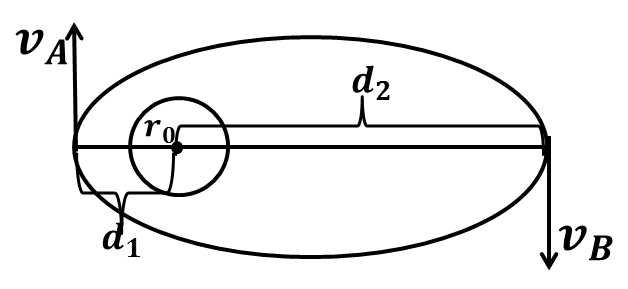
\includegraphics[height=3.5cm]{images/Lunar_orbit.jpg}
            \caption{绕月飞行轨道示意图}
            \label{fig:绕月飞行轨道示意图}
            \end{figure}
            \noindent 其中:$v_A$为近月点的速度,$v_B$为远月点速度,$r$为月球半径,$d_1$为近月点到月面的距离,$d_2$为远月点到月面的距离。
            \par
            假设只有月球对飞行器有影响。下面,我们先来求近月点和远月点的速度$v_A,v_B$。
            \par
            (1)机械能守恒定律。由于在绕月飞行阶段,飞行器不消耗燃料,故有机械能守恒:机械能 = 动能+势能。势能可以是弹性势能/重力势能。只在重力做功的情况下,物体的动能和势能之间相互转换,但总和不变
            \begin{align*}
            E_A = \frac{1}{2}mv_A^2 - \frac{GMm}{r_A}\\
            E_B = \frac{1}{2}mv_B^2 - \frac{GMm}{r_B}
            \end{align*}
            其中:$E$为机械能,$M$为月球质量,$m$为飞行器质量,$G$为万有引力常量,$r_A = r+d_1$为近月点到月心的。由机械能守恒,我们有
            \begin{align}
            \label{机械能守恒}
            E_A = E_B
            \end{align}
            \par
            (2)开普勒第二定律。1609年《新天文学》德国天文学家约翰尼斯.开普勒指出:在相等时间内,太阳和绕太阳运行的行星的连线所扫过地面积是相等的。并且该定律适用于宇宙中一切绕心的天体运动。单位时间内飞行器在近月点和远月点扫过的面积为
            \begin{align*}
            S_A = \frac{1}{2}r_A v_A\\
            S_B = \frac{1}{2}r_B v_B
            \end{align*}
            由开普勒第二定律,我们有
            \begin{align}
            \label{开普勒第二定律}
            S_A = S_B
            \end{align}
            \par
            我们要求两个参数$v_A,v_B$,就需要两个方程,组合方程(\ref{机械能守恒})和方程(\ref{开普勒第二定律})有
            \begin{align*}
            &\left\{
            \begin{aligned}
            E_A = E_B\\
            S_A = S_B
            \end{aligned}
            \right.\\
            \Rightarrow &\left\{
            \begin{aligned}
            v_A = \sqrt{\frac{2GMr_B}{r_A(r_A+r_B)}} = 1692.7m/s\\
            v_B = \sqrt{\frac{2GMr_A}{r_B(r_A+r_B)}} = 1614.4m/s
            \end{aligned}
            \right.
            \end{align*}
            其中:$M = 7350\times 10^{22}kg$,$G=6.672\times 10^{-11}N m^2/kg^2$,$r_A = r+d_1 = 1752013m$,$r_B = r+d_2 = 1837013m$。
            \par
            (3)开普勒第一定律。除了上面的这种方法之外,我们还可以寻找其他方程来求解速度$v_A,v_B$。下面,我们来介绍开普勒第一定律。开普勒在《宇宙和谐论》中表述:每一个行星都沿各自的椭圆轨道环绕太阳,而太阳则处于椭圆的一个焦点上。如图(\ref{fig:开普勒第一定律示意图})所示
            \begin{figure}[H]
            \centering
            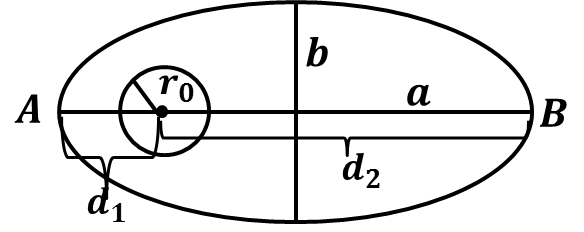
\includegraphics[height=3cm]{images/Kepler_First_Law.jpg}
            \caption{开普勒第一定律示意图}
            \label{fig:开普勒第一定律示意图}
            \end{figure}
            \par
            在图(\ref{fig:开普勒第一定律示意图})中的近月点$A$和远月点$B$处,我们有
            \begin{align*}
            \left\{
            \begin{aligned}
            & \frac{GMm}{r_A^2} = m\frac{v_A^2}{r}\\
            & r = \frac{b^2}{a}\\
            & b^2= a^2-c^2\\
            & 2a=ar_0+d_1+d_2
            \end{aligned}
            \right.\qquad
            \left\{
            \begin{aligned}
            & \frac{GMm}{r_B^2} = m\frac{v_B^2}{r}\\
            & r = \frac{b^2}{a}\\
            & b^2= a^2-c^2\\
            & 2a=ar_0+d_1+d_2
            \end{aligned}
            \right.
            \end{align*}
            其中:上面的等式用到了万有引力定律和牛顿第二定律以及椭圆的相关知识。下面我们来确定近月点和远月点的位置。
            \par
            忽略月球自转。根据该阶段所处的状态,可以大体估计出其需要的时间约为410s左右。由于嫦娥3号落点为$19.51^\circ W,44.12^\circ N$,根据假设,嫦娥三号软着陆轨道为过月球自转轴的平面,且从南至北着陆,那么嫦娥三号的近月点的维度为$44.12^\circ -12.6397^\circ = 31.4803^\circ$,即嫦娥三号近月点的经纬度为$(19.51^\circ W,31.4803^\circ N)$。根据对称性,远月点的经纬度为$(160.5^\circ E,31.4803^\circ S)$。

    \subsection{问题二的分析与求解}
        \subsubsection{问题的分析}
            \par
            确定嫦娥三号的着陆轨道和在6个阶段的最优控制策略。
        \subsubsection{模型的建立与求解}
            \par
            \textbf{(1)主减速阶段}
            \par
            主减速阶段是距离月面$15m$到$3km$,该阶段的主要任务是减速,在$3km$处速度降到$57m/s$。我们给出下面4种方案来求解此问题。
            \par
            \textbf{方案1:2D直角坐标系下的动力系统分析}。以月心为坐标系原点,以月心指向近月点(嫦娥3制动的初始点)方向为$y$轴方向,以垂直$oy$且指向娥3移动方向为$x$轴,建立平面直角坐标系$xoy$如图(\ref{fig:嫦娥3号软着陆平面直角坐标系})所示
            \begin{figure}[H]
            \centering
            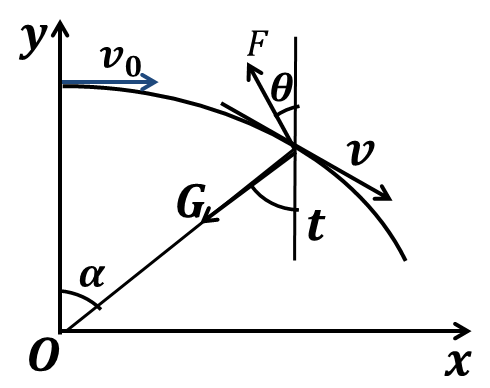
\includegraphics[height=4cm]{images/Soft_landing.jpg}
            \caption{嫦娥3号软着陆平面直角坐标系}
            \label{fig:嫦娥3号软着陆平面直角坐标系}
            \end{figure}
            \par
            以$t$时刻为研究点进行受力分析,娥3主要受月球引力$G$和主发动机制动力$F$的影响,由图(\ref{fig:嫦娥3号软着陆平面直角坐标系})中的受力分析可知
            \begin{align*}
            G &= gm\\
            &=\frac{G_0M}{r^2}m\\
            &=\frac{G_0M}{x^2+y^2}m
            \end{align*}
            且有$\alpha = \arctan\frac{x}{y}$。其中:$G_0=6.672\times10^{-1}N$为万有引力常量,$M=7.350\times 10^{22}kg$为月球质量,$m$为娥3的质量,且由于着陆过程中娥3消耗燃料制动,所以各时刻的娥3质量不同,记为$m_t$,$x,y$为坐标点、$r$为月心距皆为时变量。
            \par
            将娥3整体视为系统,我们主要关注系统在$t$时刻的系统变量:$x_t,y_t,m_t,F_t,\theta_t,v_t$。为了便于理解,不妨将时间离散化,研究系统下一时刻($t+1$时刻)的系统值。如果我们已经知道了$t$时刻的系统值,那么$t+1$时刻的系统值为
            \begin{align*}
            & x_{t+1}  =x_t + (v_{x,t+1}-v_{x,t})(t+1-t)\\
            & y_{t+1}  =y_t + (v_{y,t+1}-v_{y,t})(t+1-t)\\
            & v_{x,t+1} = v_{x,t}+a_{x,t}(t+1-t)\\
            & v_{y,t+1} = v_{y,t}-a_{y,t}(t+1-t)\\
            & a_{x,t} = \frac{F_t\sin \theta_t+G_t\sin \alpha_t}{m_t}\\
            & a_{y,t} = \frac{-F_t\cos \theta_t+G_t\cos \alpha_t}{m_t}\\
            & m_{t+1} = m_t - \frac{F_t}{v_e}\\
            & \alpha_t = \arctan \frac{x_t}{y_t}
            \end{align*}
            \par
            例如:我们给出初始值$x_0,y_0,v_0,m_0$及$F_0,\theta_0$(待求变量),即可得到系统下一时刻的状态值$x_t,y_t,v_t,m_t$。不妨将上面的离散状态更新公式写为连续时间$t$,有
            \begin{align*}
            & \dot{x} = \frac{\mathrm{d}x}{\mathrm{d}t} = v_{x,t}\\
            & \dot{y} = \frac{\mathrm{d}y}{\mathrm{d}t} = v_{y,t}\\
            & \dot{v}_x = \frac{\mathrm{d}v_x}{\mathrm{d}t} = a_{x,t}\\
            & \dot{v}_y = \frac{\mathrm{d}v_y}{\mathrm{d}t} = a_{y,t}\\
            & a_{x,t} = \frac{F_t\sin \theta_t+G_t\sin \alpha_t}{m_t}\\
            & a_{y,t} = \frac{-F_t\cos \theta_t+G_t\cos \alpha_t}{m_t}\\
            & \dot{m} = \frac{\mathrm{d}m}{\mathrm{d}t} = -\frac{F_t}{v_e}\\
            & \alpha_t = \arctan\frac{x_t}{y_t}
            \end{align*}
            由于速度是距离的导数,加速度是速度的导数,故上述系统方程可写为
            \begin{align*}
            &\ddot{x} = \frac{\mathrm{d}^2x}{\mathrm{d}t^2} = a_{x,t}\\
            &\ddot{y} = \frac{\mathrm{d}^2y}{\mathrm{d}t^2} = a_{y,t}\\
            & a_{x,t} = \frac{F_t\sin \theta_t+G_t\sin \alpha_t}{m_t}\\
            & a_{y,t} = \frac{-F_t\cos \theta_t+G_t\cos \alpha_t}{m_t}\\
            &\alpha_t = \arctan\frac{x_t}{y_t}\\
            & \dot{m} = \frac{\mathrm{d}m}{\mathrm{d}t} = -\frac{F_t}{v_e}
            \end{align*}
            \par
            最优化控制问题:从连续时间$t$来看,我们需要给出推理$F_t$和夹角$\theta_t$的函数,使系统满足初始条件$(x_0,y_0,v_0)$和终端条件$(x_t,y_t,v_t)$,并且使$t$时间消耗的能量最少;从离散时间$t$来看,我们需要给出每时刻$t$的$F_t,\theta_t$,使系统满足初始条件$(x_0,y_0,v_0)$和终端条件$(x_t,y_t,v_t)$,并且使$t$时间消耗的能量最少。上述内容可以写为如下数学模型(为和一般文献相吻合,定义0时刻为$t_0$,终止时刻为$t_f$)
            \begin{align*}
            & \min _{F,\theta} \ J = \int_{t_0}^{t_f}\dot{m}\mathrm{d}t = m_0 - m(t_f)\\
            & s.t.\left\{
            \begin{aligned}
            &x(t_0) = x_0,\ y(t_0) = y_0, \ v_x(t_0) = v_{x,0},\ v_y(t_0) = v_{y_0}, \ m(t_0) = m_0\\
            &\ddot{x} = \frac{\mathrm{d}^2x}{\mathrm{d}t^2} = a_{x,t}\\
            &\ddot{y} = \frac{\mathrm{d}^2y}{\mathrm{d}t^2} = a_{y,t}\\
            & a_{x,t} = \frac{F_t\sin \theta_t+G_t\sin \alpha_t}{m_t}\\
            & a_{y,t} = \frac{-F_t\cos \theta_t+G_t\cos \alpha_t}{m_t}\\
            &\alpha_t = \arctan\frac{x_t}{y_t}\\
            & \dot{m} = \frac{\mathrm{d}m}{\mathrm{d}t} = -\frac{F_t}{v_e}\\
            & x(t_f) = x_f,\ y(t_f) = y_f,\ v_x(t_f) = v_{x,f},\ v_y(t_f) = v_{y,f}
            \end{aligned}
            \right.
            \end{align*}
            \par
            上述优化控制的可行性:如果是在连续时间$t$上讨论上述问题,则优化控制室一个$F_t,\theta_t$的泛函问题,解$F_t,\theta_t$是无穷维的,很难求解,所以我们一般将时间$t$离散化处理。如果给定初始状态$x_0,y_0,v_0,m_0$,给定一个解$\{F_t\}_{t=t_0}^{t_f},\{\theta_t\}_{t=t_0}^{t_f}$(不妨将解何为$u = [F_t,\theta_t]^\mathrm{T},\{u_t\}_{t=t_0}^{t_f}$),根据状态更新公式(即约束条件s.t.),我们可以求解$t$时刻的系统状态$\{x_t,y_t,v_t,m_t\}$。并且要求在终端$t_f$时刻,系统状态满足要求$(x_f,y_f,v_f)$。如果有$\{u_t\}$使系统达到要求(s.t.),我们即可得到最终的目标值$J = m_0-m_f$。
            \par
            定义满足s.t.的解$\{u_t\}$为可行解,其取值域为可行域$\Phi$,故而我们可以在可行域$\Phi$中找到$\{u_t\}^*$,使得$J$最小。上面遗留的问题是:如何求解$\{y_t\}^*$。
            \par
            \textbf{方案2:2D极坐标系下的动力系统分析}。在上面的直角坐标系的处理中,我们需要使$x,y$满足$t_f$时刻的月心距要求
            \begin{align*}
            r_f= \sqrt{x_f^2+y_f^2}
            \end{align*}
            并且,要将速度$v$在各时刻$t$上分解为$v_x,v_y$。这样做虽然理解起来简单,但无疑饶了圈子,我们不妨在极坐标下对系统进行动力学分析,因为在极坐标下,$r$即为$r$,$v$与$r$方向垂直。构建2D极坐标系如图(\ref{fig:嫦娥3号软着陆平面极坐标系})所示
            \begin{figure}[H]
            \centering
            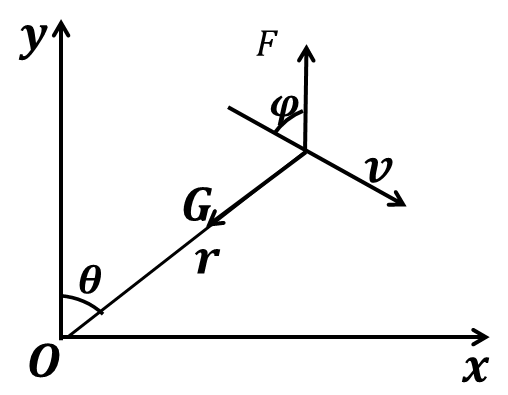
\includegraphics[height=4cm]{images/Soft_landing2.jpg}
            \caption{嫦娥3号软着陆平面极坐标系}
            \label{fig:嫦娥3号软着陆平面极坐标系}
            \end{figure}
            \par
            我们仍然假设\ding{172}不考虑其它天体对娥3的摄动;\ding{173}下降轨道与经纬线重合。我们所关心的系统变量为$(r,\theta,v,w,m,F,\varphi)$,其中:$F,\varphi$为系统控制变量;$(r,v,\theta,w,m)$为系统状态变量。
            \par
            由运动分析,我们有
            \begin{align*}
            & \dot{r} = \frac{\mathrm{d}r}{\mathrm{d}t} = v\\
            & \dot{\theta} = \frac{\mathrm{d}\theta}{\mathrm{d}t} = w
            \end{align*}
            在切向上进行受力分析,飞行器受$F\cos\varphi$及\underline{科里奥利力}的影响
            \begin{align*}
            F\cos\varphi + 2vw = -m\frac{\mathrm{d}v_y}{\mathrm{d}t}
            \end{align*}
            其中:$v_y = wr$。故有
            \begin{align*}
            \dot{w} = \frac{\mathrm{d}w}{\mathrm{d}t} = -\frac{1}{r} (\frac{F}{m} \cos\varphi+2vw)
            \end{align*}
            在径向$r$上进行受力分析
            \begin{align*}
            \left\{
            \begin{aligned}
            \frac{GMm}{r^2} = \frac{mv^2}{r}\\
            F\sin \varphi = m\frac{\mathrm{d}v}{\mathrm{d}t}
            \end{aligned}
            \right.
            \end{align*}
            其中:$v= wr$。故有
            \begin{align*}
            \dot{v} = \frac{\mathrm{d}v}{\mathrm{d}t} = \frac{F}{m}\sin \varphi - \frac{GM}{r^2}+rw^2
            \end{align*}
            \par
            由上述分析,我们得到娥3质心的运动方程为
            \begin{align*}
            & \dot{r} = \frac{\mathrm{d}r}{\mathrm{d}t} = v\\
            & \dot{v} = \frac{F}{m}\sin\varphi - \frac{GM}{r^2}+rw^2\\
            & \dot{\theta} = \frac{\mathrm{d}\theta}{\mathrm{d}t} = w\\
            & \dot{w} = -\frac{1}{r}(\frac{F}{m}\cos\varphi+2vw)\\
            & \dot{m} = -\frac{F}{v_e}
            \end{align*}
            其中:$v\in R$是娥3在矢径$r$方向上的速度;$w\in R$是娥3在角$\theta$上的角速度;$m\in R^+$是娥3质量;$G_0$为万有引力常量;$M$为月球质量;$v_e$为比冲。
            \par
            设解为$u_t = [F_t,\varphi_t]^\mathrm{T}$,离散化后可写为$\{u_t\}_{t=t_0}^{t_f}$,最优控制是寻找最优控制率$u_t^*$,使着陆过程消耗的燃料最小,并且满足初始条件和终端条件,即
            \begin{align*}
            &\min_{u=F,\varphi}\  J = \int_{t_0}^{t_f} \dot{m}\mathrm{d}t= m_0 - m(t_f) = m_0-m_f\\
            &s.t.\left\{
            \begin{aligned}
            &r(t_0) = r_0,\ v(t_0) = v_0,\ \theta(t_0) = \theta_0,\ w(t_0) = w_0,\ m(t_0) = m0\\
            & \dot{r} = \frac{\mathrm{d}r}{\mathrm{d}t} = v\\
            & \dot{v} = \frac{F}{m}\sin\varphi - \frac{GM}{r^2}+rw^2\\
            & \dot{\theta} = \frac{\mathrm{d}\theta}{\mathrm{d}t} = w\\
            & \dot{w} = -\frac{1}{r}(\frac{F}{m}\cos\varphi+2vw)\\
            & \dot{m} = -\frac{F}{v_e}\\
            & r(t_f) = r_f,\ v(t_f) = v_f,\ w(t_f) = w_f
            \end{aligned}
            \right.
            \end{align*}
            至此,主减速阶段的数学模型已经建立完毕。下面我们来讨论如何求解$\{u_t\}^*$。在此之前,先引入科里奥利力,然后再介绍求解$\{u_t\}^*$的直接法和间接法。
            \par
            \textbf{科里奥利力:}哥氏力又称科里奥利力,简称科氏力,是哥氏加速度的来源。哥氏加速度是由于质点不仅作圆周运动,还做径向运动或轴向运动所产生的。当质量为$m$的质点相对于转动参考系(月球,角速度矢量$w$)的速度为$v$时,在转动参考系内观察到科里奥利力为
            \begin{align*}
            F_c = 2mvw
            \end{align*}
            科里奥利力只有在转动参考系中运动时才发生,科氏力方向垂直相对速度,不会改变相对速度大小。
            \par
            科里奥利力的简单推导:如图(\ref{fig:科里奥利力示意图})所示
            \begin{figure}[H]
            \centering
            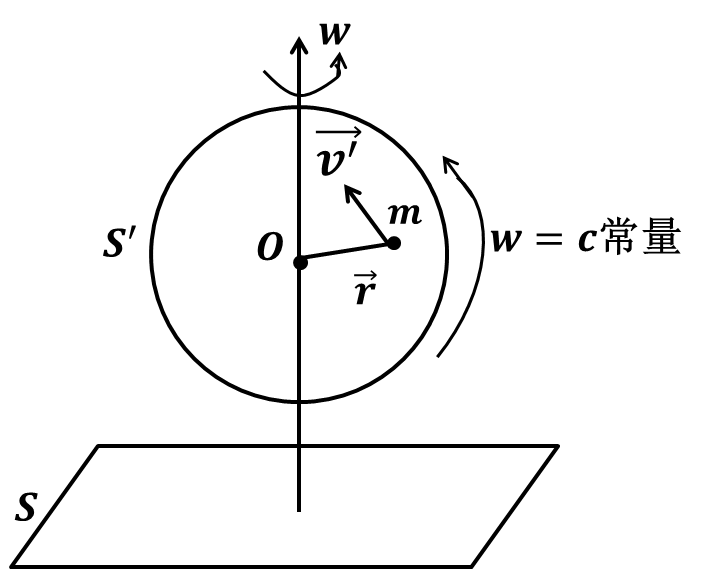
\includegraphics[height=4cm]{images/keliao.jpg}
            \caption{科里奥利力示意图}
            \label{fig:科里奥利力示意图}
            \end{figure}
            质点$m$在转动参考系$S'$中沿一光滑凹槽运动,速度为$v'$,在惯性地面$S$中
            \begin{align*}
            F = m\frac{(v^2+rw)^2}{r} = m\frac{v^2}{r}+2mv'w+mrw^2
            \end{align*}
            在非惯性系圆盘$S'$中,向心加速度为
            \begin{align*}
            a' = \frac{v'^2}{r}
            \end{align*}
            $w$的方向垂直$v$向上。
            \par
            最优控制$u_t^*$通常有2种方法:1.直接法;2.间接法。直接法是将$u_t^*$离散化、参数化后进行求解;间接法是在最优控制理论(变分/极大值原理/动态规划)的基础上,将优控问题变化为终端$t_f$自由的两点边值问题,然后求解。
            \par
            \textbf{最优控制$u_t^*$的直接法:}由于月球软着陆的轨道优化的搜索空间是一个$u_t\in \{u_t\} = R$函数空间(泛函空间),而我们通常处理的最优化问题的搜索空间是一个$\theta\in \Theta$空间(参数空间)。所以我们无法用最优化数值方法直接得到轨道,这使得我们不得不另寻它法。既然我们需要参数函数,不妨将$\{u_t\}$设为参数函数,设
            \begin{align*}
            \{u_t|u_t = u(t|\theta),\theta\in R^+\}
            \end{align*}
            例如:我们可以设$u_t$为参数多项式、傅里叶多项式等各种含参函数形式
            \begin{align*}
            u_t = \frac{1}{a+e^t}\\
            u_t = \sum_{t=0}^n a_i t^i
            \end{align*}
            这样,我们不再是在函数空间$R$中寻找一个函数$u_t^*$使$J$最优,而是在参数空间$\Theta$中寻找一个参数$\theta$,进而有$u_t^*$使$J$最优。一般文献中都使用含参多项式的形式作为$u_t$的替代,我们下面也采用这种形式。设$u_t$是一高$n$次多项式
            \begin{align*}
            u_t = \sum_{i=0}^na_it^i
            \end{align*}
            其中:$\{a_i\}_{i=0}^n = \theta\in \Theta$,共引入$n+1$个参数。
            \par
            在引入$u_t$之后,再要考虑的是:将$u_t$以连续函数的形式带入到动力方程当中进行求解,还是将时间$t$离散化逐点求解。我们先考虑将时间$t$离散化处理,将$[t_0,t_f]$离散化为$N$段,由于$t_f$不定,设
            \begin{align*}
            t_i = t_0 + \frac{i}{N}(t_f-t_0)
            \end{align*}
            其中:$N$为时间段,时间段$[t_i,t_{i+1}],i=1,2,\dots,N$的两端称为节点。这样,我们就有$i$段$[t_{i-1},t_i]$对应的$[u_{t_{i-1}},u_{t_i}]$($\{a_i\}$给定后,$u_t$对应具体数值),进而可以得到$[x_{t_{i-1}},x_{t_i}]$,进而得到$x_{t_f}$以及$J$。我们求最优$\{a\},t_f$使$J$最优。
            \par
            上述方法可以用智能算法GA等进行求解,当然,其它优化算法BFGS等亦可。而且注意到,当$F_t$为固定值时,目标变为$\min J = t_f$。在具体求解过程中,我们需要给出参数的初始值/估计值/迭代出发点。$t_f$的估计还简单一些(可以自行建模估计),但到了$\{a_i\}$却没有实际的物理意义,这使得他们的估计量是“天马行空”的。如果系统$x_t$对参数$\{a_i\}$是及其敏感的,那么,$\{a_i\}$初始估计将成为问题所在。
            \par
            问:如何解决$\{a_i\}$初始估计无依据(无物理意义)?缺:未讨论$t$不离散的情况。
            \par
            插值-分段三次埃米尔特Hermite-Simpsorn。上面,我们将时间$t$离散后,设$u_t$为多项式,那么,我们能不能假设$x_t$是多项式。承继上面的时间离散化,设$h_i=t_i-t_{i-1},i=1,2,\dots,N$,我们并不打算在$[t_0,t_f]$内设$x_t = \hat{f}(t)$,而是在某一小时间段$[t_{i-1},t_i]$进行设置,设
            \begin{align*}
            x = a_0+a_1t+a_2t^2a_3t^3 = \hat{f}(t|\theta)
            \end{align*}
            其中:$t \in [t_{i-1},t_i]$,$a$承继上面为参数$\theta$。
            \par
            也就是说,$x$在$[t_{i-1},t_i]$内皆是三次多项式,但不同时段的参数$\theta$的取值不同,即$x$为分段三次多项式。不失为一般性,我们在时段$[t_0,t_1]$内研究$x$。
            \begin{align}
            \label{直接法:三次多项式}
            & x = a_0+a_1t+a_2t^2a_3t^3 \\
            & t\in [t_0,t_1]\notag
            \end{align}
            假设我们知道了以下条件
            \begin{align}
            \label{4个已知条件}
            & x(t_0) = x_0\notag\\
            & x(t_1) = x_1\notag\\
            & x'(t_0) = x_0' = f(x_{t_0})\notag\\
            & x'(t_1) = x_1' = f(x_{t_1})
            \end{align}
            其中:$\dot{x} = f(x_t,u_t,t)$。当$x_0$给定后,只要有$u_0$即有$x_0'$。那么,我们就可以在$[t_0,t_1]$区间内对函数$x(t)$进行插值,例如用三次Hermite多项式插值($[t_0,t_f]$段上即为分段三次Hermite多项式插值)。
            \par
            注:关于插值的数值分析技术,可以参考《数值分析》李乃成P127.
            \par
            式(\ref{直接法:三次多项式})有四个参数待求,而我们有4个已知条件(\ref{4个已知条件}),我们可以利用解方程组的形式求解参数$a_i$
            \begin{align*}
            \begin{bmatrix}
            x_1\\
            \dot{x}_1\\
            x_2\\
            \dot{x}_2
            \end{bmatrix}
            =
            \begin{bmatrix}
            1 & 0 & 0 & 0 \\
            0 & 1 & 0 & 0 \\
            1 & 1 & 1 & 1 \\
            0 & 1 & 2 & 3
            \end{bmatrix}
            \begin{bmatrix}
            a_0\\
            a_1\\
            a_2\\
            a_3
            \end{bmatrix}
            \end{align*}
            解上述方程组即可得到$\{a_i\}_{i=0}^3$,将$a_i$带入到$H$三次多项式有
            \begin{align*}
            H_3(t) = \hat{x}(t) & =  \left( 1+2\frac{t_0-t}{t_0-t_1} \right) \left( \frac{t-t_1}{t_0-t_1} \right) ^2 + \left( 1+2\frac{t_1-t}{t_1-t_0} \right) \left( \frac{t-t_0}{t_1-t_0} \right) ^2x(t_1)\\
            & \quad + (t-t_0) \left( \frac{t-t_1}{t_0-t_1} \right) ^2x'(t_0)+(t-t_1) \left( \frac{t-t_0}{t_1-t_0} \right) ^2 x'(t_1)
            \end{align*}
            其中:$t_1-t_0 = h_1$,$\dot{x} = f(x,u,t)$。
            \par
            这样,我们就得到了$[t_0,t_1]$区间内$x(t)$的Hermite插值估计$H_3(t)$。但是,由于我们需要求解$x_0,x_1,u_0,u_1$,每给一组$(x_0,x_1,u_0,u_1)$,都会有一个$H_3(t)$与之对应,$x_0,x_1,u_0,u_1$取不同值时的$H_3(t)$示意图如图(\ref{fig:x-0等取不同值时的H-3示意图})所示
            \begin{figure}[H]
            \centering
            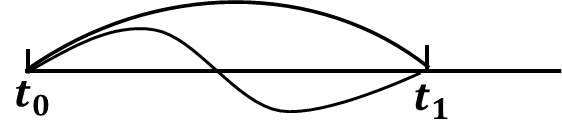
\includegraphics[width=5cm]{images/x_0H_3.jpg}
            \caption{x-0等取不同值时的H-3示意图}
            \label{fig:x-0等取不同值时的H-3示意图}
            \end{figure}
            \par
            既然有这么多$H_3(t)$,那么我们需要约束$H_3(t)$,不能让其乱跑。我们用条件$\dot{x} = f(x,u,t)$来进行约束。任给$t\in [t_0,t_1]$,$u(t)$给定后,如果知道$x(t)$,则$\dot{x}(t)$是知道的,$H_3(t),H'_3(t)$是已知的。我们可以在$[t_0,t_1]$内取$k$个点$\{t_k\}$,要求这$k$个点的$H'_3(t)$和$\dot{x}(t) = f(H_3(t),u(t),t)$相等或者近似(配点)。为计算简单,这里$k=1$,置$t_k = \frac{t_0+t_1}{2}$(当$k$越大点数越多时,计算越精确,但计算量会相应变大)
            \begin{align*}
            H_3(t_k) = \frac{x_0+x_1}{2}+\frac{h_1}{8}(f_0-f_1)\\
            H_3'(t_k) = -\frac{3(x_0-x_1)}{2h_1} - \frac{f_0-f_1}{4}
            \end{align*}
            其中:$\dot{x}_0= f(x_0,u_0,t_0) = f_0$,$\dot{x}_1 = f(x_1,u_1,t_1) = f_1$。
            \par
            在给出$u_k$后,要求$H_3'(t_k) = \dot{x}(t_k)$,这里我们两种方案。方案(1),我们利用$H_3(t_k)$直接替代$x(t_k)$,有
            \begin{align*}
            H'_3(t_k) = \dot{x}(t_k) = f(H_3(t_k),u(t_k),t_k)
            \end{align*}
            方案(2),三阶Simpson方法然后再用$H_3(t_k)$直接替代$x(t_k)$,区间$[a,b]$上的三阶Simpson求积公式如下
            \begin{align*}
            S_i = \frac{b-a}{6}[f(a)+4f(\frac{a+b}{4})+f(b)]
            \end{align*}
            结合上面的三阶Simpson求积公式,我们有
            \begin{align*}
            & x_{i+1} = x_i + \frac{h_i}{6}[f(x_i,u_i,t)+4f(H_3(t_k),u(t_k),t_k)+f(x_{i+1},u_{i+1},t_{i+1})]\\
            & x_1 = x_0 + \frac{h_1}{6}[f(x_0,u_0,t_0)+4f(H_3(t_k),u(t_k),t_k)+f(x_{1},u_{1},t_{1})]
            \end{align*}
            注:$x$为$f(t)$,$H_0 = x_0 = x(0),H_1=x_1=x(1)$一定是高度重合的。
            \par
            经过上面的分析,在$[t_0,t_1]$时段内的处理我们已经基本完成,很容易将上述结论推广到$N$段。在$[t_0,t_1]$段内,我们假设已知$(x_0,x_1,\dot{x}_0,\dot{x}_1,u_{t_k})$,故这样变为我们需要求解的优化变量,由于$\dot{x}$与$u$有关,故我们需要求解的优化变量为
            \begin{align*}
            z = [x_0^\mathrm{T},u_{c0}^\mathrm{T},u_0^\mathrm{T},x_1^\mathrm{T},u_{c1}^\mathrm{T},u_1^\mathrm{T},\dots,x_N^\mathrm{T},u_{cN}^\mathrm{T},u_N^\mathrm{T}]
            \end{align*}
            其中:$u_{ci}^\mathrm{T}$即为第$[t_{i-1},t_i]$段内的配点$t_k$的控制量。
            \par
            这种方法将最优控制问题离散化、参数化后,转化为非线性规划问题,如下
            \begin{align*}
            & \min_z \ J = \int_{t_0}^{t_f}\dot{m}\mathrm{d}t = -m(t_f)\\
            & s.t.\left\{
            \begin{aligned}
            & r(0) = r_0,\ v(0) = v_0,\ \theta(0) = 0,\ w(0) = w_0,\ m(0) = m_0\\
            & u_{min} \leqslant u \leqslant u_{max}\\
            & \dot{x} = f(x,u,t)\\
            & r(t_f)=r_f,\ v(t_f) = v_f,\ w(t_f) = 0
            \end{aligned}
            \right.
            \end{align*}
            \par
            上述s.t.并不易于书写,我们来捋一下:\ding{172}首先,哪些是待优化变量?
            \begin{align*}
            z = [x_0^\mathrm{T},u_{c0}^\mathrm{T},u_0^\mathrm{T},x_1^\mathrm{T},u_{c1}^\mathrm{T},u_1^\mathrm{T},\dots,x_N^\mathrm{T},u_{cN}^\mathrm{T},u_N^\mathrm{T}]
            \end{align*}
            将$[t_0,t_f]$等分为$N = 20$段,共$21$个节点。各节点上有5个状态变量$x$,2个控制变量$u$。20段中的中间配点有2个$u$($k=1$),故待优化变量个数为
            \begin{align*}
            (N+1)(n_x+n_u)+N(n_u)
            \end{align*}
            其中:$n_x$为$x$变量个数;$n_u$为$u$变量个数,$N$为段数。\ding{173}等式约束。上面的优化模型中的等式约束是
            \begin{align*}
            \text{初始条件+终端条件}+(Nn_x)\text{的HS等式约束}
            \end{align*}
            \ding{174}不等式约束为
            \begin{align*}
            & u_{min} \leqslant (N+1)n_u \leqslant u_{max}\\
            & u_{min} \leqslant (N)n_u \leqslant u_{max}
            \end{align*}
            \par
            承继上面的想法,能否直接给出$(x_i,x_{i+1},u_i,u_{i+1})$,并设置一定的等式条件。文\cite{Sun.2006}利用4阶R-K(Runge-Kutta)法实现了直接法。这里我们给出R-K公式(可以参考\cite{Li}P273、\cite{Hu}P9、\cite{Chen}P141),考虑如下一阶常微分初值问题
            \begin{align*}
            \left\{
            \begin{aligned}
            & y'(x) = f(x,y(x))\\
            & y(a) = y_0
            \end{aligned}
            \right.
            \end{align*}
            上述问题的4阶R-K计算公式为
            \begin{align*}
            \left\{
            \begin{aligned}
            & y_{i+1} = y_i + \frac{1}{6}(K_1+2K_2+2K_3+K_4)\\
            & K_1 = hf(x_i,y_i)\\
            & K_2 = hf(x_i+\frac{1}{2}h,y_i+\frac{1}{2}K_1)\\
            & K_3 = hf(x_i+\frac{1}{2}h,y_i+\frac{1}{2}K_2)\\
            & K_4 = hf(x_i+h,y_i+K_3)
            \end{aligned}
            \right.
            \end{align*}
            其中:$h$为$x$的步长。改进的4阶R-K公式为
            \begin{align*}
            \left\{
            \begin{aligned}
            & y_{i+1} = y_i + \frac{1}{6}(K_1+4K_3+K_4)\\
            & K_1 = hf(x_i,y_i)\\
            & K_2 = hf(x_i+\frac{1}{2}h,y_i+\frac{1}{2}K_1)\\
            & K_3 = hf(x_i+\frac{1}{2}h,y_i+\frac{1}{4}K_1+\frac{1}{4}K_2)\\
            & K_4 = hf(x_i+h,y_i-K_2-2K_3)
            \end{aligned}
            \right.
            \end{align*}
            以及
            \begin{align*}
            \left\{
            \begin{aligned}
            & y_{i+1} = y_i + \frac{1}{8}(K_1+3K_2+3K_3+K_4)\\
            & K_1 = hf(x_i,y_i)\\
            & K_2 = hf(x_i+\frac{1}{3}h,y_i+\frac{1}{3}K_1)\\
            & K_3 = hf(x_i+\frac{2}{3}h,y_i-\frac{1}{3}K_1+K_2)\\
            & K_4 = hf(x_i+h,y_i+K_1-K_2+K_3)
            \end{aligned}
            \right.
            \end{align*}
            \par
            承继上面的$[t_0,t_f]$离散化方法,并且有系统状态方程
            \begin{align*}
            \dot{x} = f(x,u,t)
            \end{align*}
            在区间$[t_{i_1},t_i],i=1,2,\dots,N(t_N = t_f)$,假设我们有$(x_{i-1},u_{i-1},x_i,u_i)$,那么由4阶R-K,我们有$x_{i-1},x_i$的计算公式
            \begin{align*}
            x_i = x_{i-1}+\frac{1}{6}(K_1+2K_2+2K_2+K_4)
            \end{align*}
            其中:
            \begin{align*}
            \left\{
            \begin{aligned}
            & K_1 = h_kf(x_k,u_k,t_k)\\
            & K_2 = h_kf(x_i+\frac{1}{2}K_1,\bar{\lambda}_{k+1},\bar{t})\\
            & K_3 = h_kf(x_i+\frac{1}{2}K_2,\bar{\lambda}_{k+1},\bar{t})\\
            & K_4 = h_kf(x_i+K_3,\bar{\lambda}_{k+1},t_{k+1})\\
            & h_k = t_{k+1}-t_k,\ h_{i-1} = t_i - t_{i-1},\ i=1,2,\dots,N\\
            & \bar{t} = \frac{1}{2}(t_k+t_{k+1})\\
            & \lambda_{k+1} = \lambda(\bar{t})
            \end{aligned}
            \right.
            \end{align*}
            经过上述离散化处理后,原优化控制问题变为非线性规划问题,其优化变量为
            \begin{align*}
            z = [x_0,u_0,x_1,u_1,\dots,x_N,u_N]^\mathrm{T}
            \end{align*}
            \par
            上面两种方法都将最优控制问题处理为含约束的非线性规划问题,处理非线性规划问题的方法有很多,可以参考前面相应的章节。非线性规划的处理方法一般有:1.可行方向法;2.罚函数法(内点法);3.梯度投影法;4.逐步二次规划SQP。而MATLAB主要采用SQP方法。
            \par
            \textbf{最优控制$u_t^*$的间接法:}跋山涉水,终于到了最优控制$u_t^*$的间接解法(后面,我们还会建立软着陆的3D动力系统)。前面,我们花了很大篇幅来讨论系统$\dot{x} = f(x,u,t)$,泛函$J(x_t,u_t,t)$。泛函极值存在条件是欧拉方程、最优控制中的控制量$u_t$无约束时的变分法、控制量$u_t$有约束时的P极大值原理及动态规划。下面,我们就要用这些理论来分析娥3轨道的优化问题。
            \par
            我们可以看出,娥3轨道最优控制问题是一个控制量$u = (F,\varphi)$有约束且约束$t_f$自由、$x(t_f)$有约束的最优控制问题,因此,我们可以用P极大值原理或动态规划进行求解。下面,我们将用P极大值原理求解最优控制$u^* = (F,\varphi)^*$,利用P极大值原理求解最优控制律$u_t^*$,从而将问题转化为两点边值问题,当然也可以进行离散化求解。
            \par
            1962.Kriegsman和Reiss利用变分法求解最优控制律$u_t$。2000年王大秩等利用Pontryagin极大值原理求解$u_t$,将问题转变为两点边值问题,并用一种初值猜测的打靶算法进行求解。2004年,单永正等利用Pontryagin极大值原理,将问题转化为两点边值问题,并将两点边值问题转化为非线性规划问题进行求解。2004年,赵松吉等利用初值猜测技术和线性摄动求解两点边值问题。
            \par
            下面,我们用Pontryagin极大值原理求解最优控制律$u_t = (F_t,\varphi_t)^\mathrm{T}$。记
            \begin{align*}
            f(x,u,t) =
            \left[
            \begin{aligned}
            & f_1 = v\\
            & f_2 = \frac{F}{m}\sin\varphi - \frac{G_0M}{r^2}+rw^2\\
            & f_3 = w\\
            & f_4 = -\frac{1}{r}(\frac{F}{m}\cos\varphi+2vw)\\
            & f_5 = -\frac{F}{v_e}
            \end{aligned}
            \right]
            \end{align*}
            于是动力系统方程可以写为
            \begin{align*}
            \dot{x} = f(x,u,t) = f(x(t),u(t),t)
            \end{align*}
            \par
            (1)引入拉格朗日乘子/共轭变量$\lambda = [\lambda_r,\lambda_v,\lambda_\theta,\lambda_w,\lambda_m]^\mathrm{T}$,构建$H$(哈密顿函数)
            \begin{align*}
            H(x,\lambda,u,t) & = \lambda^\mathrm{T}f(x,u,t)\\
            & = \lambda_r f_1+\lambda_vf_2+\lambda_\theta f_3+\lambda_wf_4+\lambda_m f_5\\
            & = \frac{F}{mr} \left( r\lambda_v\sin \varphi-\lambda_w\cos\varphi-\frac{\lambda_m}{v_e}mr \right) +H_2\\
            & = H_1(F,\varphi)+H_2
            \end{align*}
            其中:$H_2$表示与控制变量$F,\varphi$无关部分。由P极大值原理,有$\max H \triangleq \max H_1$。
            \par
            (2)写正则方程,有
            \begin{align*}
            & \dot{\lambda} = -\frac{\partial H}{\partial x} (= 0)\\
            & \dot{x} = -\frac{\partial H}{\partial \lambda} (= 0) = f(x,u,t)
            \end{align*}
            推得
            \begin{align*}
            & \dot{\lambda}_r = -\frac{2\lambda_v G_0M}{r^3} - \lambda_v w^2 - \frac{\lambda_w F\cos\varphi}{mr^2} - 2\lambda_w vw\\
            & \dot{\lambda}_v = \frac{2w\lambda_w}{r} - \lambda_r\\
            & \dot{\lambda}_\theta = 0\\
            & \dot{\lambda}_w = \frac{2v\lambda_w}{r} - \lambda_\theta-2rw\lambda_v\\
            & \dot{\lambda}_m = \frac{\lambda_vF\sin\varphi}{m^2} - \frac{\lambda_w F\cos\varphi}{rm^2}
            \end{align*}
            \par
            (3)写控制方程,有
            \begin{align*}
            \dot{u} = \frac{\partial H}{\partial u}(=0)
            \end{align*}
            \par
            (4)终端约束
            \begin{align*}
            G = \left[
            \begin{aligned}
            r(t_f) = r_f\\
            v(t_f) = v_f\\
            w(t_f) = w_f
            \end{aligned}
            \right] = 0
            \end{align*}
            \par
            (5)横截条件
            \begin{align*}
            \lambda(t_f) = \left[\frac{\partial J}{\partial x}+\frac{\partial G}{\partial x}r  \right]_{t = t_f}
            \end{align*}
            其中:$r$为拉格朗日乘子。
            \par
            (6)控制律约束
            \begin{align*}
            F_{min} \leqslant F_i \leqslant F_{max}\\
            \varphi_{min} \leqslant \varphi_i \leqslant \varphi_{max}
            \end{align*}
            \par
            由于求$u$上的极值,令控制方程等于0
            \begin{align*}
            \dot{u} = \frac{\partial H}{\partial u}=0
            \end{align*}
            有$\varphi,F$的最优控制律
            \begin{align*}
            & \varphi^* = -\arctan \left( \frac{\lambda_v r}{\lambda_w} \right) \\
            & F^* = \left\{
            \begin{aligned}
            & F_{max} \quad s(t) >0\\
            & 0\quad s(t)<0
            \end{aligned}
            \right.
            \end{align*}
            其中:$s(t)=\frac{\lambda_v \sin \varphi}{m} - \frac{\lambda_w \cos\varphi}{mr} - \frac{\lambda_m}{v_e} $。
            \par
            在求解最优控制律$u_t^*$后,要求$x^*,\lambda^*$使$H$最大。将$u_t^*$带入正则方程当中,利用初始条件和终端条件对正则方程积分,即可求出最优$x^*,\lambda^*$,此时,问题转化为微分方程中的两点边值问题。
            \par
            简单分析一下,在离散化下考虑,在$x(t_0)$已知的情况下,给定一个初始值$\lambda(t_0)$,我们会得到相应的最优控制律$u(t_0)^*$,进而由$\dot{x} = f$得到$x(t_1)$。依次迭代,可以得到终端$x(t_f) = x_f$(在给定初始$t_f$后)。进一步观察$\lambda_m$的取值,对$\lambda_{/m}$及$x$没有影响,因此,只要先选取迭代初始值$[\lambda_r,\lambda_v,\lambda_w]_{t=t0}$,确定$u_{t_0}$,再给出已知$x(t_0) = x_0$。在正则方程上积分,即可得到末端状态$x(t_f)$,即$x(t_f)$是初值$[\lambda_r,\lambda_v,\lambda_w]_{t=t0},t_f$的函数,进而性能$J$也是是$(\lambda_r(t0),\lambda_v(t0),\lambda_w(t0),t_f)$的函数。这样,两点边值问题就被离散化为非线性规划(只有等式约束)。
            \par
            迭代初始值$t_f$可以根据一定的公式进行估计,文\cite{Zhao}给出估计
            \begin{align*}
            t_f &= \frac{\Delta m}{|\dot{m}|} = \frac{\Delta m}{F/v_e}\\
            & = \frac{m_0 [1-\exp (-\Delta v/v_eg)]}{F/v_e}\\
            & = \frac{m_0[1-\exp(-\sqrt{r_0^2+2gh}/v_eg)]}{F/v_e}
            \end{align*}
            其中:$|\dot{m}|$为发动机燃料秒耗量。
            \par
            但是迭代初始值$(\lambda_r(t0),\lambda_v(t0),\lambda_w(t0),t_f)$的选取则没有那么多依据,我们只能凭空设置。如果正则方程对初始值仍然敏感,那么$(\lambda_r(t0),\lambda_v(t0),\lambda_w(t0))$将成为问题的所在。下面的“伴随-控制”变换可以解决这一问题。设
            \begin{align*}
            \lambda_v(t_0) r_0 = \sin (\varphi_0)\\
            \lambda_w(t_0) = -\cos(\varphi_0)
            \end{align*}
            将$\tan\varphi =- \frac{\lambda_v r}{\lambda_w}$对$t$求导,有
            \begin{align}
            \label{嫦娥3号:公式1}
            \frac{\dot{\varphi}}{\cos^2\varphi} = - \left[ \frac{\dot{\lambda}_vr}{\lambda_w}+\frac{\lambda_vr}{\lambda_w} - \frac{\lambda_v r\dot{\lambda}_w}{\lambda_w^2} \right]
            \end{align}
            将正则方程和$\lambda_v^0,\lambda_w(t_0)$带入式(\ref{嫦娥3号:公式1}),有
            \begin{align*}
            \lambda_r = \frac{\dot{\varphi}}{\lambda_wr}+\frac{2\lambda_w w}{r}-\frac{\lambda_v v}{r}+\frac{2\lambda_v r w}{\lambda_w}
            \end{align*}
            于是有
            \begin{align*}
            \lambda_r(t_0) = \frac{\dot{\lambda}}{\lambda_w(t_0)r_0} + \frac{2\lambda_w(t_0)w_0}{r_0} - \frac{\lambda_v(t_0)v_0}{r_0}+\frac{2\lambda_v(t_0)r_0w_0}{\lambda_w(t_0)}
            \end{align*}
            这样,$(\lambda_r(t0),\lambda_v(t0),\lambda_w(t0))$就可以用$\varphi_0,\dot{\varphi}_0$替代,可以取合理的初始值了。
            \par
            \textbf{引:两点边值问题的数值解}。考虑下面一个简单的二阶常微分方程的两点边值问题
            \begin{align*}
            \left\{
            \begin{aligned}
            & y''(x) = f(x,y,y')\\
            & y(a) = y_a\\
            & y(b) = y_b\\
            & a<x<b
            \end{aligned}
            \right.
            \end{align*}
            前面我们讨论了常微的初值问题,我们能不能在初值问题的基础上求解边值问题?能,但对于二阶常微的初值$y(a) = \Delta_1,y'(a) = \Delta_2$,我们还不足以求解边值问题,我们缺少一个条件。那我们就设一个条件好了,我们设$y'(z) - m$,并舍去$y(b)=y)b$,有
            \begin{align*}
            \left\{
            \begin{aligned}
            & y''(x) = f(x,y,y')\\
            & y(a) = y_a\\
            & y''(a) = m
            \end{aligned}
            \right.
            \end{align*}
            \par
            数值求解上述两点边值问题。一个正常的思路是,我们不断调整$m$,使$y(b) = y_b$,如图(\ref{fig:两点边值问题的打靶方法})所示
            \begin{figure}[H]
            \centering
            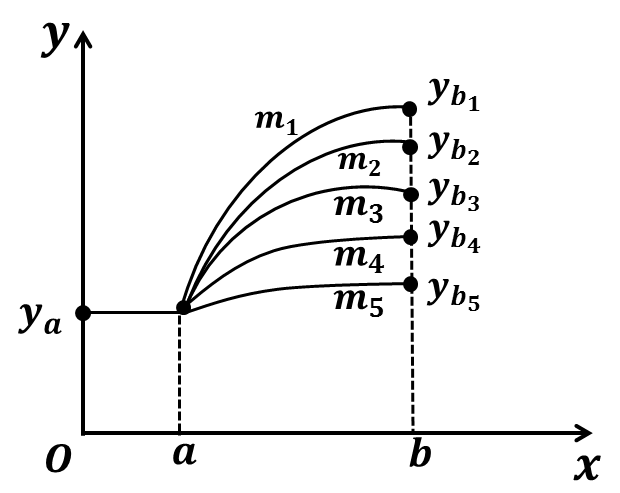
\includegraphics[height=4cm]{images/two_point.jpg}
            \caption{两点边值问题的打靶方法}
            \label{fig:两点边值问题的打靶方法}
            \end{figure}
            两点边值问题的打靶方法算法伪代码如(\ref{code:2点边值打靶法ode})所示
            \begin{algorithm}[htbp]
                \caption{2点边值打靶法ode}\label{code:2点边值打靶法ode}
                \begin{algorithmic}[1]
                    \State 初始化:$m$,$\varepsilon$,$t_{max}$,$i:=0$。
                    \While {$t=1,2,\dots,t_{max}$}
                        \State $//$解初值问题
                        \begin{align*}
                        \left\{
                        \begin{aligned}
                        & y''(x) = f(x,y,y')\\
                        & y(a) = y_a\\
                        & y''(a) = m_i
                        \end{aligned}
                        \right.
                        \end{align*}
                        \State $\beta _i = y(b)$。
                        \If {$|\beta_i-\beta|>\varepsilon$}
                            \State 修正$m_{i+1}$。
                        \EndIf
                    \EndWhile
                \end{algorithmic}
            \end{algorithm}
            \par
            上述伪代码中遗留的问题是:如何修正$m$。理想的$m$是$y(b,m) = y_b$,但在数值求解过程中,不存在解析表达式,并不易解。一种可行的方式是取
            \begin{align*}
            m_2= \frac{y_b}{y_{b1}}m_1
            \end{align*}
            此后,由非线性方程求根的割线法更新$m_i$
            \begin{align*}
            m_i = m_{i-1} - \frac{y(b,m_{i-1}) - y_b}{y(b,m_{i-1}) - y(b,m_{i-2})}(m_{i-1}- m_{i-2}) \quad i=3,4,\dots
            \end{align*}
            \par
            Matlab中的ode45用于求解初值问题,bvp4c用于求解边值问题。注:由于状态变量的量级差异大,在轨道积分过程中会导致有效位数的损失,归一化处理可以克服这一缺点。在一般论文中皆有归一化说明,这里就不做叙述了。
            \par
            \textbf{方案3:3D球面坐标系下的动力系统分析。}很明显的一个问题是:我们用上面的方案1或者方案2中的2D动力学模型只能做某一方向上的平移,而不能做平面上的移动。而题中既然给了空间上的数字高程图,那我们就有必要在3维空间中建立着陆轨道。当然,我们可以在未拍照之前的主减速阶段和快速调整阶段建立2D模型,在拍照之后建立3D模型,但这无疑增加了复杂性。幸运的是,3D模型的建立和求解与2D模型是相似的。
            \par
            如前面2D分析的那样,我们要考虑的问题是:1.在直角坐标系下建模还是在球面坐标系下建模;2.是否考虑月球自转;3.用直接法还是间接法求解最优控制问题。3D球面坐标系下的动力学模型如图(\ref{fig:3D球面坐标系下的动力学模型})所示
            \begin{figure}[H]
            \centering
            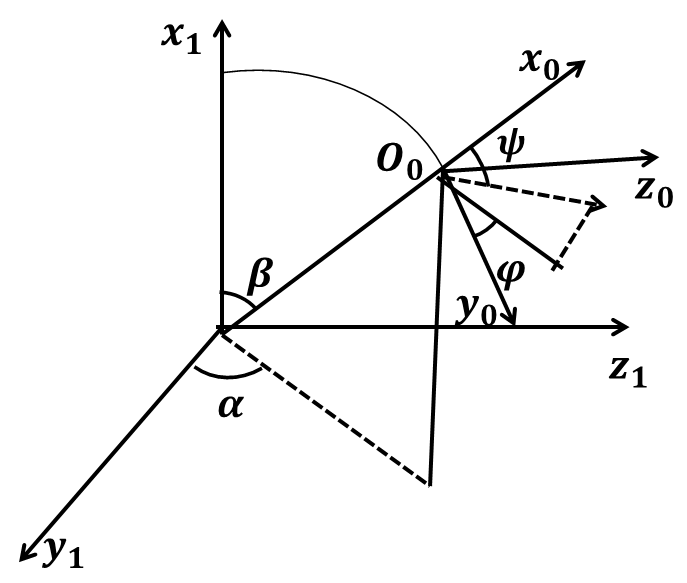
\includegraphics[height=4cm]{images/3D_Spherical.jpg}
            \caption{3D球面坐标系下的动力学模型}
            \label{fig:3D球面坐标系下的动力学模型}
            \end{figure}
            \par
            假设:1.忽略月球自转;2.月球引力场为均匀引力场,$g$为常值;3.不考虑其他星体对娥3的摄动。以月心$o_1$为坐标原点,$\overrightarrow{o_1x_1}$指向近月点(娥3下降点),$\overrightarrow{o_1y_1}$指向娥3着陆方向,$\overrightarrow{o_1z_1}$按右手法则确定,建立月心惯性坐标系$o_1x_1y_1z_1$。$o_0o_1$为娥3到月心的距离$r$,$\alpha$为$o_0o_1$在$y_1o_1z_1$面投影与$\overrightarrow{o_1y_1}$正方向夹角,$\beta$为$o_0o_1$与$\overrightarrow{o_1x_1}$正方向夹角,由此有球面坐标系$(r,\alpha,\beta)$。
            \par
            此外,我们还需要确定推力$F$的方向。以娥3质心$o_0$为原点,$\overrightarrow{o_0x_0}$为背月心$\overrightarrow{o_1o_0}$延长线,$\overrightarrow{o_0y_0}$指向娥3运行方向,$\overrightarrow{o_0z_0}$由右手法则确定。建立着陆轨道坐标系$o_0x_0y_0z_0$,$\psi,\varphi$为推力$F$的方向角,形成球面坐标系$(F,\psi,\varphi)$。
            \par
            在上面的假设下,月球软着陆的动力学方程可以表示为
            \begin{align*}
            \ddot{\vec{a}} = \ddot{\vec{r}} = \frac{\vec{F}}{m} - \frac{\vec{r}}{\vec{r}^3}G_0M
            \end{align*}
            其中:$\ddot{\vec{r}}$是娥3的加速度矢量,$\vec{F}$为发动机动力矢量,$\vec{r}$为娥3的位移矢量,$G_0$为万有引力常量,$M$为月球质量。不妨令$G_0M = \mu$(常量)。
            \par
            将位移矢量$\vec{r}$按$o_0x_0y_0z_0$方向轴分解为$r_x,r_y,r_z$;将$\vec{r}$按$o_1x_1y_1z_1$方向轴分解为$r_x',r_y',r_z'$。通过$o_0x_0y_0z_0$我们可以看到,$o_0x_0y_0z_0$沿$o_0x_0$轴逆方向转动$(90-\alpha)^\circ$,然后沿$o_0y_0$轴逆时针转动$\beta$,最后沿$o_0z_0$轴顺时针转动$(90-\alpha)^\circ$即可与$0_1x_1y_1z_1$归正。因此,从着陆轨道坐标系$o_0x_0y_0z_0$转到月心惯性坐标系$o_1x_1y_1z_1$的转动矩阵$I$为
            \begin{align*}
            I = \begin{bmatrix}
            \cos\alpha\cos\beta& \sin \beta& -\sin \alpha\cos\beta\\
            -\cos\alpha\sin\beta & \cos\beta& \sin\alpha\sin\beta\\
            \sin\alpha&0&\cos\alpha
            \end{bmatrix}
            \end{align*}
            即$[r_x',r_y',r_z']^\mathrm{T} = I[r_x,r_y,r_z]^\mathrm{T}$。
            \par
            对娥3质心$o_0$沿$o_1x_1y_1z_1$各方向轴进行受力分析,用$a_z,a_y,a_z$表示各方向轴的加速度,有
            \begin{align*}
            & \ddot{r} -\dot{\alpha}^2 r\sin ^2\beta - \dot{\beta}^2r=a_x\\
            & 2\dot{\beta}\dot{r}+\ddot{\beta}r-\dot{\alpha}^2r\cos\beta\sin \beta = a_y\\
            & 2\dot{\alpha}\dot{r}\sin \beta + \ddot{\alpha}r\sin \beta + 2\dot{\alpha}\dot{\beta}r\cos\beta = a_z\\
            & a_x = \frac{F\cos\psi}{m} - \frac{\mu}{r^2}\\
            & a_y = \frac{F\sin\psi\cos\varphi}{m}\\
            & a_z = \frac{F\sin\psi\sin\varphi}{m}\\
            & \dot{m} = -\frac{F}{v_e}
            \end{align*}
            \par
            用$v_x,v_y,v_z$表示速度$v$在$o_1x_1y_1z_1$各方向轴的分量,化简上述方程,有
            \begin{align*}
            & \dot{r} = v_x\\
            & \dot{\beta} = \frac{v_y}{r}\\
            & \dot{\alpha} = \frac{v_z}{r\sin \beta}\\
            & \dot{v}_x = \frac{F\cos\psi}{m} - \frac{\mu}{r^2} + \frac{v_y^2+v_z^2}{r}\\
            & \dot{v}_y = \frac{F\sin\psi\cos\varphi}{m} - \frac{v_xv_y}{r}+\frac{v_z^2}{r\tan\beta}\\
            & \dot{v}_z = \frac{F\sin \psi\sin\varphi}{m} - \frac{v_xv_y}{r}-\frac{v_yv_z}{r\tan\beta}\\
            & \dot{m} = -\frac{F}{v_e}
            \end{align*}
            其中:$\mu = G_0$为常量,$v_e$为发动机比冲常量。由此,我们得到了3D球面坐标系下的轨道运动方程(系统)。
            \par
            \textbf{方案4:3D直角坐标系下的动力系统分析。}在直角坐标系下对系统进行受力分析是简单的。设$v_x,v_y,v_z$沿用上面的设置,则有
            \begin{align*}
            \dot{x} = v_x\\
            \dot{y} = v_y\\
            \dot{z} = v_z
            \end{align*}
            设$v_x',v_y',v_z'$为速度$v$在$o_0x_0y_0z_0$各方向轴分量,则有
            \begin{align*}
            & \dot{v}_x' = \frac{F\cos\psi}{m} - \frac{\mu}{r^2}\\
            & \dot{v}_y' = \frac{F\sin\psi\cos\varphi}{m}\\
            & \dot{v}_z' = \frac{F\sin\psi\sin\varphi}{m}
            \end{align*}
            同时,由坐标转换有
            \begin{align*}
            [\dot{v}_x,\dot{v}_y,\dot{v}_z] = I[\dot{v}_x',\dot{v}_y',\dot{v}_z']
            \end{align*}
            于是,3D直角坐标系下的动力方程(系统)为
            \begin{align*}
            & \dot{x} = v_x\\
            & \dot{y} = v_y\\
            & \dot{z} = v_z\\
            & \dot{v}_x' = \frac{F\cos\psi}{m} - \frac{\mu}{r^2}\\
            & \dot{v}_y' = \frac{F\sin\psi\cos\varphi}{m}\\
            & \dot{v}_z' = \frac{F\sin\psi\sin\varphi}{m}\\
            & [\dot{v}_x,\dot{v}_y,\dot{v}_z] = I[\dot{v}_x',\dot{v}_y',\dot{v}_z']\\
            & \dot{m} = -\frac{F}{v_e}
            \end{align*}
            \par
            文献\cite{Zhou}建立了3D直角坐标系且考虑了月球自转的着陆动力系统。在上面不考虑月球自转的前提下,我们建立了软着陆的3D直角坐标系和球面坐标系下的动力系统。下面,我们给出此动力系统的最优控制模型。
            \par
            设$x= [r,\beta,\alpha,v_x,v_y,v_z,m]^\mathrm{T}$为系统的状态变量,$u = [F,\psi,\varphi]$为系统的控制变量,设$\dot{x} = f(x,u,t)$为系统的状态方程,其中$f$为标量函数。我们的目标是控制$u$,使系统消耗燃料最少,故娥3的最优控制模型为
            \begin{align*}
            & \min_u \ J = \int_{t_0}^{t_f}\dot{m}\mathrm{d}t = m_0 - m_f\\
            & s.t.\left\{
            \begin{aligned}
            & r(t_0) = r_0,\ \beta(t_0) = \beta_0,\ \alpha(t_0) = \alpha_0,\\
            & v_x(t_0) = v_{x0},\ v_y(t_0) = v_{y0},\ v_z(t_0) = v_{z0},\ m(t_0) = m_0\\
            & \dot{x} = f(x,u,t)\\
            & r(t_f) = r_f,\ \beta(t_f) = \beta_f,\ \alpha(t_f) = \alpha_f,\ v_x(t_f) = v_{xf},\ v_y(t_f) = v_{yf},\ v_z(t_f) = v_{zf}\\
            & F_{min} \leqslant F <F_{max}\\
            & \varphi_{min} \leqslant \varphi \leqslant \varphi_{max}\\
            & \psi_{min} \leqslant \psi \leqslant \psi_{max}
            \end{aligned}
            \right.
            \end{align*}
            其中:$J$为积分型指标泛函。
            \par
            上述最优控制问题是一个终端给定、$t_f$不定、系统状态含约束、控制函数$u$含约束的积分型最优控制问题。像分析2D最优控制那样,其解法可分为直接法和间接法。(1)直接法:我们可以将$[t_0,t_f]$离散化后,将泛函最优控制问题转化为参数最优化问题进行求解。(2)间接法:利用P极大值原理,将最优控制问题转化为两点边值问题,继而可以用打靶算法和离散化参数化优化算法进行求解。哈工大.张仲满2009.6硕士论文中提到用PID自适应网络求解上述最优控制问题,同时讨论了P极大值原理+殆尽的打靶算法在该问题中的应用;哈工大.单永正.2009.7博士论文中提到用参数化技术+约束变换额方法来参数化求解最优控制问题,文中给出了相应的理论与算法,并用miser3.2最优控制软件进行求解;哈工大.张锋.2009.6硕士论文中分析了姿态发动机的姿态控制,并用Lyapunov分析系统稳定性,提出在软着陆末端进行姿态发动机和主减速发动机联合控制策略;关于模糊、灰色、随机系统的最优控制问题可以参考葛宝明,林飞《先进控制理论》。由于3D动力系统的求解和2D系统相似,这里,我们不再继续3D求解工作。
            \par
            \textbf{(2)快速调整阶段}
            \par
            \par
            \textbf{(3)粗避障阶段}
            \par
            在减速阶段和快速调整阶段之后,娥3进入粗避障和精避障阶段。粗避障阶段的范围是月面2.4km到100m区间,其主要目的是避开大的陨石坑,实现在设计着陆点上方100m处悬停,并初步确定落月地点。嫦娥3号在月面2.4km时,对正下方$2300\times 2300m$的范围进行拍照,获得数字高程地图如图(\ref{fig:距2400m处的数字高程图})。
            \par
            下面,我们将利用数字高程图中的信息来建立避障模型。由于拍摄区域相对月球很小,不妨假设地面为水平,不考虑月球弧度。以娥3所在位置俯视月面,进行拍摄,以其右下方顶点为$o$点,以高程图$0$高度水平面为$xoy$面,建立直角坐标系如图(\ref{fig:避障坐标系})所示。其中:$(x_0,y_0)$为嫦娥3在月面正下方投影,图中阴影表示陨石坑,圆叉表示山峰。由于是数字高程图,我们可以得到$2300\times 2300$中各点的高度,不妨设各点高度为$h(x_i,y_j),i,j=1,2,\dots,n$,$n$为行像素点个数。
            \begin{figure}[H]
            \centering
            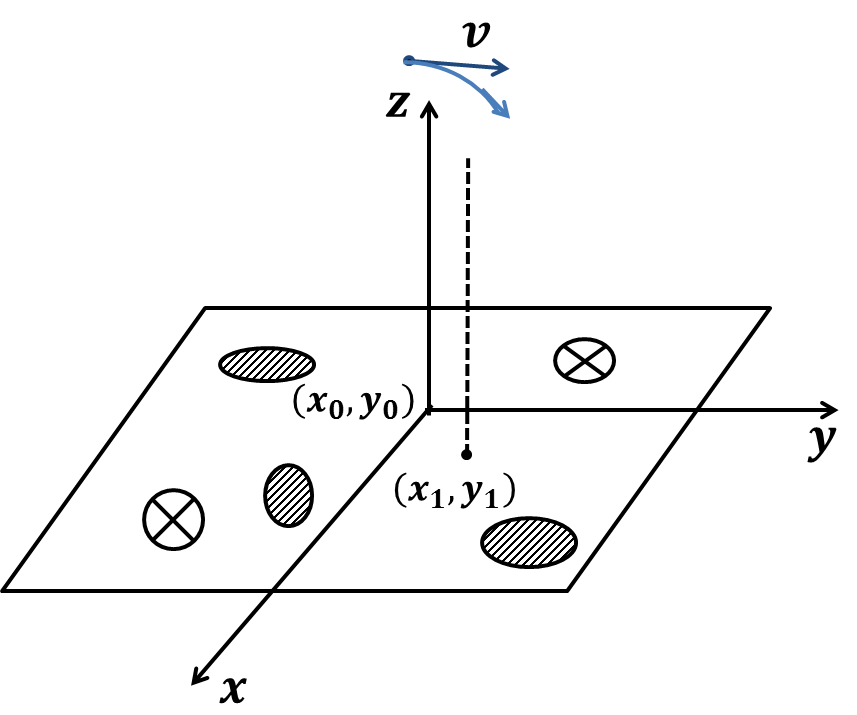
\includegraphics[height=4cm]{images/Obstacle_avoidance_coordinate_system.jpg}
            \caption{避障坐标系}
            \label{fig:避障坐标系}
            \end{figure}
            \par
            由于地面上有许多噪声,我们不妨在进行选择区域之间对图像进行去噪处理。之后,我们考虑着陆点的条件,我们应该综合这些信息来评价某一点$(x_i,y_j)$。我们考虑以下3个评价指标:
            \begin{enumerate}
            \item 点$(x_i,y_j)$应该平缓;
            \item 点$(x_i,y_j)$平缓且其所在地区也具有一定的平缓度;
            \item 点$(x_i,y_j)$应该距离$(x_0,y_0)$不远,以避免消耗较多燃料。
            \end{enumerate}
            \par
            我们在$(x_i,y_j)$中找到最优着陆点为$(x_1,y_1)$。我们有了上述3个评价之后,接下来的工作就是量化指标,并构建评价函数。我们应该逐点$(x_i,y_j)$来考虑问题,即给出每个点的评价值,并从中选优,而不是划大的区域,那样我们找不到一个确定的点来指导娥3着陆。
            \par
            (一)着陆区平缓性指标。首先,$(x_i,y_j)$只有在靠近水平面上时,才平缓一点,也就是说,高度$h_i$较大较小都不好。我们可以用$h_i$的分布来看一下$h_i$的情况。其次,与平缓最接近的数学定义是梯度。我们用Sobel算子计算高程图的梯度函数$S(x,y)$,并进行降噪处理,颜色越深地区越平坦。定义平稳性因子为
            \begin{align*}
            P(x,y) = |h|+S(x,y)
            \end{align*}
            $P(x,y)$越小越好。
            \par
            (二)着陆区耗能型指标。点$(x_i,y_j)$距离$(x_0,y_0)$越远,则所耗能量越多。不妨设置耗能函数为
            \begin{align*}
            F(x,y) = (x-x_0)^2+(y - y_0)^2
            \end{align*}
            (三)着陆区广阔性指标。由于飞行器娥3具有一定的大小/体积,并且在控制下落过程中,有许多误差的干扰,会导致着陆点并不是很准确,所以我们需要着陆点具有一定的广阔性。以着陆点$(x_i,y_j)$为圆心,$r_i$为半径的区域内的平均平缓都要在
            \begin{align*}
            D(x,y) = \mathrm{E}(p|r)
            \end{align*}
            \par
            对于一个地点$(x_i,y_j)$的评价要综合上述3点。我们设置3个指标的权重为$\lambda_1,\lambda_2,\lambda_3$,则最终个的评价指标函数为
            \begin{align*}
            A(x,y) = \lambda_1 P(x,y)+\lambda_2F(x,y)+\lambda D(x,y|r)
            \end{align*}
            \par
            \textbf{(4)精避障阶段}
            \par
            精避障阶段的区间是月面100m到30m,要求娥3悬停在100m处时对着陆区100m范围内进行拍摄,并获取三维数字高程图,如图(\ref{fig:距月面100m处的数字高程图})所示。分析三维数字高程图,避开大的陨石坑,确定最终着陆点,实现在着陆上方30m处水平方向速度为0$m/s$。
            \par
            我们介绍一种基于李雅普诺夫稳定控制理论的非线性方法。李雅普诺夫控制制导法主要利用李雅普诺夫稳定理论来进行控制律$u$的求解。下面介绍李雅普诺夫稳定判定定律
            \begin{theorem}[李雅普诺夫稳定判定定律]
            \par
            设系统状态方程为
            \begin{align*}
            \dot{x} = f(x,u,t)
            \end{align*}
            其中:$f(0,0,t) = 0$。如果存在一具有连续一阶偏导数的标量函数(即李雅普诺夫函数)$v(x,u,t)$,并且满足
            \begin{align*}
            v(x,u,t)\text{为正定}\\
            \dot{v}(x,u,t)\text{为负定}
            \end{align*}
            则状态空间原点处的平衡状态是一致渐进稳定的。
            \end{theorem}
            \par
            选取正定的李氏函数$v$,要求李氏函数$v$即能表示当前位置危险程度,又能表示距离着陆点的位置关系。这样,$v$函数就代表了飞行器娥3的期望性能。令他的导数为负,求取控制律,可以保证飞行器的状态达到期望位置(即使系统在期望状态处是一只渐进稳定的)。在月球精避障阶段(100m-30m),控制律的目的是保证娥3在指定的高度(30m)处平移到安全着陆点上方。飞行器平移的初始点为悬停点(100m),其末端点位于安全着陆点上方(30m),并且希望飞行器到达着陆点上方时的平移速度为0。
            \par
            要求正定的李氏函数$v$,即能表示当前状态/位置危险程度,又能表示到预定着陆点的燃料消耗情况,故构建由能量函数和势危函数组成的$v$,如下:\ding{172}能量函数
            \begin{align}
            \label{能量函数}
            \phi_p(x,y,z,\dot{x},\dot{y},\dot{z}) = [x-x_0,y-y_0,z-z_0,\dot{x},\dot{y},\dot{z}]
            \begin{bmatrix}
            p_1&0&0&0&0&0\\
            0&p_2&0&0&0&0\\
            0&0&p_3&0&0&0\\
            0&0&0&1&0&0\\
            0&0&0&0&1&0\\
            0&0&0&0&0&1
            \end{bmatrix}
            \begin{bmatrix}
            x-x_0\\
            y-y_0\\
            z-z_0\\
            \dot{x}\\
            \dot{y}\\
            \dot{z}
            \end{bmatrix}
            \end{align}
            其中:$(x,y,z)$表示飞行器在$oxyz$下的位置,$(x_0,y_0,z_0)$表示平移末端点,$(x_0,y_0,0)$为安全着陆点,$z_0$为指定高度($z_0 = 100 - 30$),$(\dot{x},\dot{y},\dot{z}) = (v_x,v_y,v_z)$表示速度$v$的方向分量。在平移末端期望该状态量为0。飞行器的$(x,y,z,\dot{x},\dot{y},\dot{z})$由系统状态给出,$x_0,y_0$由安检系统给出,$z_0$事先给定,$p_1,p_2,p_3\in R^+$,函数$\phi_p$越大,则距离着陆点$(x_0,y_0)$越远,速度偏差越大。
            \par
            \ding{173}势危函数为
            \begin{align}
            \label{势危函数}
            \phi_s(x,y) = \sum_{i=1}^n|z_i| e^{ -\frac{(x-x_i)^2+(y-y_i)^2}{\sigma^2}  }
            \end{align}
            其中:$x,y$表示娥3的$x,y$轴位置,$(x_i,y_i,z_i)$为障碍物位置、高度/深度,$i$为障碍物需要,共$n$个障碍物,$\sigma$为超参,代表了危险威胁范围,$\sigma$越大,障碍物对周围的危险越大。$\phi_s$越大,则越危险。
            \par
            上面给出了能量函数(\ref{能量函数})和势危函数(\ref{势危函数}),由此,我们可以设置李雅普诺夫函数
            \begin{align*}
            v = \phi(x,y,z,\dot{x},\dot{y},\dot{z}) = \phi_p+k_1\phi_s
            \end{align*}
            其中:$k_1$为权重参数。由$\phi_p,\phi_s$为正定,有$\phi>0$,并且$\phi$为状态$x(t)$的函数。由李雅普诺夫第二定理可知:当$\phi<0$时,则系统在状态空间平衡点出的平衡状态是一致渐进稳定的,该平衡点记为$v$的极小点。
            \par
            下面给出李雅普诺夫最优控制律。李雅普诺夫函数的导数为三个方向周速度的函数,并且负定。此方法可以保证娥3到达平移末端时,其水平速度为0,即令$\dot{\phi} = -k_x\dot{x}^2-k_y\dot{y}^2-k_z\dot{z}^2$,其中:$k_x,k_y,k_z$为正数。由于$\phi$为$(x,y,z\dot{x},\dot{y},\dot{z})$的函数,所以$\frac{\mathrm{d}\phi}{\mathrm{d}t}$可以由链式法则求出
            \begin{align*}
            \frac{\mathrm{d}\phi}{\mathrm{d}t} =&  \frac{\partial \phi}{\partial x}\frac{\partial x}{\partial t}+\frac{\partial \phi}{\partial y}\frac{\partial y}{\partial t}+\frac{\partial \phi}{\partial z}\frac{\partial z}{\partial t}+ \frac{\partial \phi}{\partial \dot{x}}\frac{\partial \dot{x}}{\partial t}+\frac{\partial \phi}{\partial\dot{y}}\frac{\partial \dot{y}}{\partial t}+\frac{\partial \phi}{\partial \dot{z}}\frac{\partial \dot{z}}{\partial t}\\
            =& \frac{\partial \phi}{\partial x}\dot{x}+\frac{\partial \phi}{\partial y}\dot{y}+\frac{\partial \phi}{\partial z}\dot{z}+\frac{\partial \phi}{\partial \dot{x}}\ddot{x}+\frac{\partial \phi}{\partial \dot{y}}\ddot{y}+\frac{\partial \phi}{\partial \dot{z}}\ddot{z}
            \end{align*}
            \par
            下面,我们来求解$\frac{\partial \phi}{\partial x},\frac{\partial \phi}{\partial \dot{x}},\frac{\partial \phi}{\partial y},\frac{\partial \phi}{\partial \dot{y}},\frac{\partial \phi}{\partial z},\frac{\partial \phi}{\partial \dot{z}}$
            \begin{align*}
            & \frac{\partial \phi}{\partial x}  = 2p_1(x-x_0) - \frac{2}{\sigma^2}\sum_{i=1}^n k_1|z_i|(x-x_i) e^{ -\frac{(x-x_i)^2+(y-y_i)^2}{\sigma^2}  }\\
            & \frac{\partial \phi}{\partial y}= 2p_2(y-y_0) - \frac{2}{\sigma^2}\sum_{i=1}^n k_1|z_i|(y-y_i) e^{ -\frac{(x-x_i)^2+(y-y_i)^2}{\sigma^2}  } \\
            & \frac{\partial \phi}{\partial z}= 2p_3(z-z_0) \\
            & \frac{\partial \phi}{\partial \dot{x}} =2\dot{x} \\
            & \frac{\partial \phi}{\partial \dot{y}}=2\dot{y} \\
            & \frac{\partial \phi}{\partial \dot{z}}=2\dot{z}
            \end{align*}
            \par
            注:含月球自转的着陆器质心运动方程为
            \begin{align*}
            \ddot{r} = u+\mu-2w\dot{r}-w(w(r+\rho))
            \end{align*}
            其中:$r$为位置矢量,$u$为旋转角速度,$u$为控制量,$\mu = G_0M$。月球自转角速度$w = 2.66\times 10^{-6}rad/s$所带来的向心力和科氏力较小,所以我们前面将其忽略了。由于着陆末端飞跨的纬度较小,所以设月球引力场为均匀引力场。$g = \frac{G_0M}{r^2}$为常量。
            \par
            下面,我们来求$(\dot{x},\dot{y},\dot{z},\ddot{x},\ddot{y},\ddot{z})$。$(\dot{x},\dot{y},\dot{z},\ddot{x},\ddot{y},\ddot{z})$即为质心运动方程,由前面的3D直角坐标系下的动力系统给出。
            前面的3D直角坐标系下的动力系统为
            \begin{align*}
            & \dot{x} = v_x\\
            & \dot{y} = v_y\\
            & \dot{z} = v_z\\
            & \ddot{x} = \dot{v}_x = \frac{F_1\cos\phi}{m} - \frac{\mu}{r^2} + \frac{v_y^2+v_z^2}{r}+\frac{F_{2x}}{m}\\
            & \ddot{y} = \dot{v}_y = \frac{F_1\sin\phi\cos\varphi}{m} - \frac{v_xv_y}{} + \frac{v_z^2}{r\tan\beta}+\frac{F_{2y}}{m}\\
            & \ddot{z} = \dot{v}_z = \frac{F_1\sin\phi\sin\varphi}{m} - \frac{v_xv_y}{} - \frac{v_yv_z}{r\tan\beta}+\frac{F_{2z}}{m}\\
            &\dot{m} = -\frac{F_1+F_2}{m}
            \end{align*}
            其中:$F_{2x},F_{2y},F_{2z}$为姿态发动机推力$F_2$在个方向上的分量。由此,我们的得到$\frac{\mathrm{d}\phi}{\mathrm{d}t}$。下面我们对运动方程进行简化。
            \par
            由于在着陆末端$[100-0]m$处,$\beta\to \frac{\pi}{2},\tan \beta \to \infty$,并且,要考虑姿态发动机的调整作用,我们对娥3重新进行受力分析,以简化$\ddot{x},\ddot{y},\ddot{z}$。
            \par
            娥3在末端主要有3个作用力:\ding{172}主发动机推力$F_1$;\ding{173}姿态发动机调整力$F_2$;\ding{173}月球引力$\frac{G_0Mm}{r^2} = \mu m$。我们将3者的合力设为$F = F_1+F_2+G$,设$F$在月心坐标系下各方向轴所产生的加速度为$a_x,a_y,a_z$,则
            \begin{align*}
            \ddot{x} = a_x = F_x/m = (\vec{F}_{1x}+\vec{F}_{2x}+\vec{G}_x)/m\\
            \ddot{y} = a_y = F_y/m = (\vec{F}_{1y}+\vec{F}_{2y}+\vec{G}_y)/m\\
            \ddot{z} = a_z = F_z/m = (\vec{F}_{1z}+\vec{F}_{2z}+\vec{G}_z)/m
            \end{align*}
            为使$\dot{x} = -k_x\dot{x}^2-k_y\dot{y}^2+k_z\dot{z}^2$恒成立,可以得到$x,y,z$各方向轴的期望加速度$\ddot{x},\ddot{y},\ddot{z}$为
            \begin{align*}
            & \ddot{x} = -k_x \frac{\dot{x}}{2}+\sum_{i=1}^nk_1|z_i|e^{-\frac{(x-x_i)^1+(y-y_i)^2}{\sigma^2}} \frac{x-x_i}{\sigma^2} - p_1(x-x_0)\\
            & \ddot{y} = -k_y \frac{\dot{x}}{2}+\sum_{i=1}^nk_1|z_i|e^{-\frac{(-x_i)^1+(y-y_i)^2}{\sigma^2}} \frac{y-y_i}{\sigma^2} - p_2(y-y_0)\\
            & \ddot{z} = \frac{\mu}{r} - k_z\frac{\dot{z}}{2}- p_3(z-z_0)
            \end{align*}
            其中:$k_1,k_x,k_y,k_z,p_1,p_2,p_3$为参数。下面我们来简化运动方程:如果按上面的运动方程进行求解,我们还需要得到控制量$u = [F,\psi,\varphi,F_{2x},F_{2y},F_{2z}]^\mathrm{T}$的李雅普诺夫最优控制律。这样就太麻烦了。
            \par
            考虑到末端$\beta\to \frac{\pi}{2}$,并且飞行器娥3并不会偏离$oy$轴太远,即$\alpha\to \frac{\pi}{2}$,月球引力常量$G$可进行化简
            \begin{align*}
            G \approx [G_x,G_y,G_z]^\mathrm{T} = [G\cos\beta,G\sin\beta\cos\alpha,G\sin\beta\sin\alpha]^\mathrm{T}
            \end{align*}
            有
            \begin{align*}
            \lim_{\substack{\alpha\to \pi/2\\\beta\to \pi/2}} G(\alpha,\beta) = [G_x,G_y,G_z]^\mathrm{T} = [0,0,G]^\mathrm{T}
            \end{align*}
            说明:上式说明月球引力常量$G$只牵引娥3沿$z$轴向月心运动。
            \par
            并且,我们考虑到主发动机推理$F_1$与$z$轴方向重合($\psi=\pi/2,\varphi=\pi/2$),且姿态发动机在娥3周围(底部和上部没有),于是
            \begin{align*}
            \left\{
            \begin{aligned}
            & F_{1x} = 0,\ F_{1y} = 0,\ F_{1z} = F_1\\
            & F_{2z} = 0
            \end{aligned}
            \right.
            \end{align*}
            说明:上式说明主发动机$F_1$方向与$z$轴重合,即发动机主要指引娥3进行$z$方向的降落;姿态发动机$F_2$在$z$方向合力为0,主要指引娥3进行$xoy$平移。所以,简化后的运动方程为
            \begin{align*}
            & \ddot{x} = a_x = F_{2x}/m\\
            & \ddot{y} = a_y = F_{2y}/m\\
            & \ddot{z} = a_z = F_{1z}/m - G/m = F_{1z}/m - \mu
            \end{align*}
            因此,化简后的控制律记为$u=[F_1,F_{2x},F_{2y}]^\mathrm{T}$,可以由期望控制律(期望加速度)$\ddot{x},\ddot{y},\ddot{z}$求出。该控制律$u$是在李雅普诺夫控制理论下求取的,故其可以保证李雅普诺夫稳定。
            \par
            飞行器娥3在月面100m处悬停,并进行拍照,$x_0 = (0,0,100),v_0=(0,0,0)$。取能量函数加权系数$p_1=p_2=p_3=0.002$,势危函数权重$k_1=0.1$,形状系数$\sigma^2=2$,势函数下降函数$k_x=k_y=k_z= 0.2$。
            \par
            todo:结果图:能量函数图、势危函数图、李氏函数图、在李高程图中避障轨迹、$v_x,v_y,v_z,x,y,z$曲线。
            \par
            讨论:$z_i$的确定;注:PUPF调节器、PID神经网络控制(假设采用连续姿态推理),当然,如果不考虑姿态发动机,以$[F,\psi,\varphi]^\mathrm{T}$替代亦可。
            \par
            \textbf{(5)缓速下降阶段}
            \par
            缓速下降阶段的主要任务是控制飞行器在$4m$时的速度为0,之后关闭发动机,娥3以自由落体着陆到指定点,其示意图如图(\ref{fig:缓速下降阶段示意图})所示
            \begin{figure}[H]
            \centering
            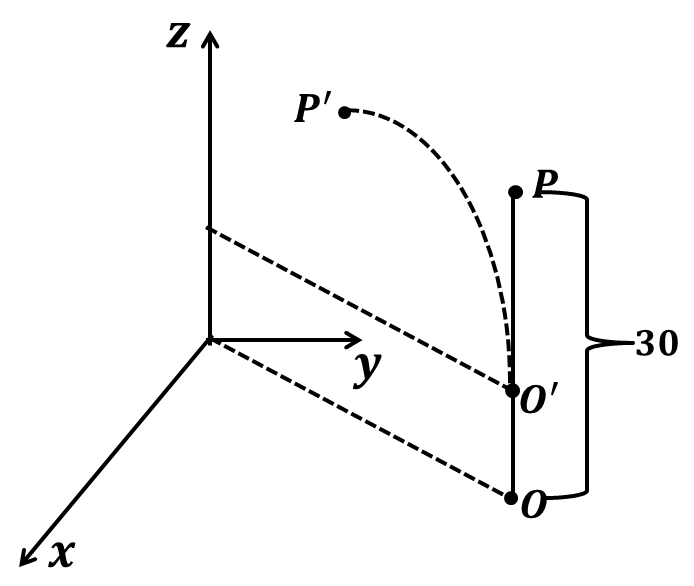
\includegraphics[height=4cm]{images/slow_down.jpg}
            \caption{缓速下降阶段示意图}
            \label{fig:缓速下降阶段示意图}
            \end{figure}
            \par
            如果娥3在30m出时,能准确降落到$P$点($P$点位着陆点$o$的正上方30m处),那么缓速下降的模型可以简化为古老的(经典)软着陆问题。例如:《现代控制理论及应用》齐晓慧P155。缓速下降阶段的运动方程为
            \begin{align*}
            & \dot{z} = v\\
            & \dot{v} = \frac{\mu}{r^2} - \frac{F}{m}\\
            & \dot{m} = -\frac{F}{v_e}
            \end{align*}
            其中:$z$为月心坐标系下的$z$轴值,即高度值,$v$为速度。并且假设姿态调整力$F_2$为0,推力$F_1$方向与$z$轴重合。
            \par
            上述系统的状态量为$x = [z,v,m]^\mathrm{T}$,控制量$u = F$。建立以燃料消耗最小为性能指标的积分型最优控制模型如下
            \begin{align*}
            & \min_u\ J = \int_{t_0}^{t_f} \dot{m}(t)\mathrm{d}t\\
            & s.t.\left\{
            \begin{aligned}
            & x(0) = x_0\\
            & \dot{x} = f(x,u,t)\\
            & x(t_f) = x_f\\
            & u_{min} \leqslant u \leqslant u_{max}
            \end{aligned}
            \right.
            \end{align*}
            \par
            但是,由于实际情况(误差原因)飞行器在30m时不能达到$P$点而是达到$P'$,因此,我们仍要在3维空间中进行分析,并且还要考虑姿态发动机的存在,以实现高精度着陆工作。
            \par
            承继前面的$F_1$和$F_2$的假设,假设$F_1$的方向与$z$轴重合,$F_2$仅产生$F_{2x},F_{2y}$两个方向上的分力,以简化模型。我们有简化后的系统动力学模型
            \begin{align*}
            & \dot{x} = v_x\\
            & \dot{y} = v_y\\
            & \dot{z} = v_z\\
            & \dot{v}_x = F_x/m\\
            & \dot{v}_y = F_y/m\\
            & \dot{v}_z = \mu/r^2 - F_1/m\\
            & \dot{m} = \frac{F_1+F_2}{v_e}
            \end{align*}
            最优控制目标仍然为燃料消耗最少,可用适当的方法进行求解。
            \par
            注:哈工大.张锋.2009硕士论文中给出了姿态联合动力系统,并用参数化+强化技术+约束变换进行最优控制律的求解,并于着陆末端,在姿态耦合系统的基础上求解系统的联合镇定控制律。

    \subsection{问题三的分析与求解}
        \subsubsection{问题的分析}
            \par
            对于你们设计的着陆轨道和控制策略做相应的误差分析和敏感性分析。
        % \subsubsection{模型的建立与求解}

% \bibliography{change3hao}%bib文件名称
% \end{document}
